\chapter{Finite Differences}
%Finite difference schemes are very much similar to trinomial tree options pricing, where each node is dependent on three other nodes with an up movement, a down movement, and a flat movement.
 
A common method to numerically solve Ordinary Differential Equations (ODE), like heat equation, Black-Scholes equation, etc\ldots is the finite difference method, where finite difference formulas at evenly spaced grid points can be used to approximate the differential equations. This way, a differential equation is transformed into a system of algebraic equations to solve.
An ordinary differential equation is a differential equation containing one or more functions of one independent variable and the derivatives of those functions~\cite{bib:ode}. The term ordinary is used in contrast with the term partial differential equation which may be with respect to more than one independent variable.

\section{Finite Difference Method}

In the finite difference method, the derivatives in the differential equation are approximated using the finite difference formulas. Imagine to divide the interval of $[a,b]$ into $n$ equal sub-intervals of length $h$ as shown in Figure~\ref{fig:finite_difference_1}.

\begin{figure}[htb]
	\centering
	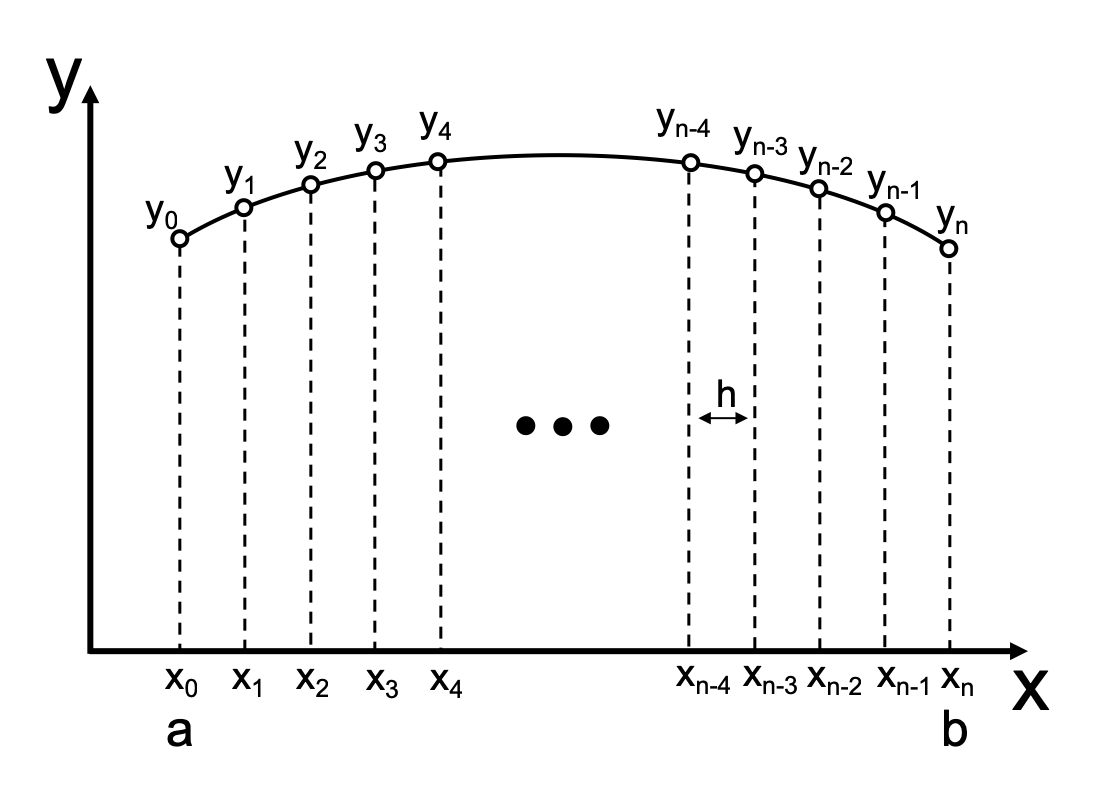
\includegraphics[width=0.7\textwidth]{figures/finite_difference_1}
	\caption{Example of grid used to solve an Ordinary Differential Equation.}
	\label{fig:finite_difference_1}
\end{figure} 

Commonly, we usually use the central difference formulas in the finite difference methods due to the fact that they yield better accuracy. The differential equation is enforced only at the grid points, and the first and second derivatives are:

\begin{equation}
\cfrac{\partial y}{\partial t} = \cfrac{y_{i+1}−y_{i−1}}{2h}
\end{equation}

\begin{equation}
\cfrac{\partial^2y}{\partial t^2} = \cfrac{\cfrac{\partial y_{i+1}}{\partial t} - \cfrac{\partial y_{i-1}}{\partial t}}{h} = \cfrac{\cfrac{y_{i+1}−y_{i}}{h} - \cfrac{y_{i}−y_{i−1}}{h}}{h}=\cfrac{y_{i−1}−2y_i+y_{i+1}}{h^2}
\end{equation}

These finite difference expressions are used to replace the derivatives of $y$ in the differential equation which leads to a system of $n+1$ linear algebraic equations if the differential equation is linear. If the differential equation is nonlinear, the algebraic equations will also be nonlinear.

As an example imagine we are going out to launch a rocket, and let $y(t)$ be the altitude (meters from the surface) of the rocket at time $t$. We know the gravity $g=9.8$~m/s$^2$. If we want to have the rocket at $50$~m off the ground after 5 seconds after launching, what should be the velocity at launching? 
The ODE we need to solve is 

\begin{equation*}
\cfrac{\partial^2y}{\partial t^2} = -g
\end{equation*}

with the boundary conditions $y(0)=0$ and $y(5)=50$. Let’s take $n=10$, so let's make a grid with ten steps in time.

Since the time interval is $[0,5]$ and we have chosen $n=10$, $h=0.5$, using the finite difference approximated derivatives, we have

\begin{gather*}
y0=0 \\
y_{i−1}−2y_i+y_{i+1}=−gh^2,i=1,2,...,n−1\\
y_{10}=50
\end{gather*}

If we use matrix notation, we will have:
\begin{equation*}
\begin{bmatrix}
1 & 0\\
1 & -2 & 1 \\
  &  \ddots & \ddots & \ddots & \\
  & &  1 & -2 & 1 \\
  &  &  &  & 1 
\end{bmatrix}
\begin{bmatrix}
y_0 \\
y_1 \\
\vdots \\
y_{n-1} \\
y_n 
\end{bmatrix}
=
\begin{bmatrix}
0\\
-gh^2 \\
\vdots \\
-gh^2 \\
50
\end{bmatrix}
\end{equation*}

Therefore, we have 11 equations in the system, that can be solved using the method explained in Chapter~\ref{matrix-equations}.

\begin{ipython}
import numpy as np
import matplotlib.pyplot as plt

n = 10
h = (5-0) / n

# Get A
A = np.zeros((n+1, n+1))
A[0, 0] = 1
A[n, n] = 1
for i in range(1, n):
    A[i, i-1] = 1
    A[i, i] = -2
    A[i, i+1] = 1

print(A)

# Get b
b = np.zeros(n+1)
b[1:-1] = -9.8*h**2
b[-1] = 50
print(b)

# solve the linear equations
y = np.linalg.solve(A, b)

t = np.linspace(0, 5, 11)

plt.figure(figsize=(10,8))
plt.plot(t, y)
plt.plot(5, 50, 'ro')
plt.xlabel('time (s)')
plt.ylabel('altitude (m)')
plt.show()
\end{ipython}
\begin{ioutput}
[[ 1.  0.  0.  0.  0.  0.  0.  0.  0.  0.  0.]
 [ 1. -2.  1.  0.  0.  0.  0.  0.  0.  0.  0.]
 [ 0.  1. -2.  1.  0.  0.  0.  0.  0.  0.  0.]
 [ 0.  0.  1. -2.  1.  0.  0.  0.  0.  0.  0.]
 [ 0.  0.  0.  1. -2.  1.  0.  0.  0.  0.  0.]
 [ 0.  0.  0.  0.  1. -2.  1.  0.  0.  0.  0.]
 [ 0.  0.  0.  0.  0.  1. -2.  1.  0.  0.  0.]
 [ 0.  0.  0.  0.  0.  0.  1. -2.  1.  0.  0.]
 [ 0.  0.  0.  0.  0.  0.  0.  1. -2.  1.  0.]
 [ 0.  0.  0.  0.  0.  0.  0.  0.  1. -2.  1.]
 [ 0.  0.  0.  0.  0.  0.  0.  0.  0.  0.  1.]]
[ 0.   -2.45 -2.45 -2.45 -2.45 -2.45 -2.45 -2.45 -2.45 -2.45 50.  ]
\end{ioutput}

\begin{figure}[htb]
	\centering
	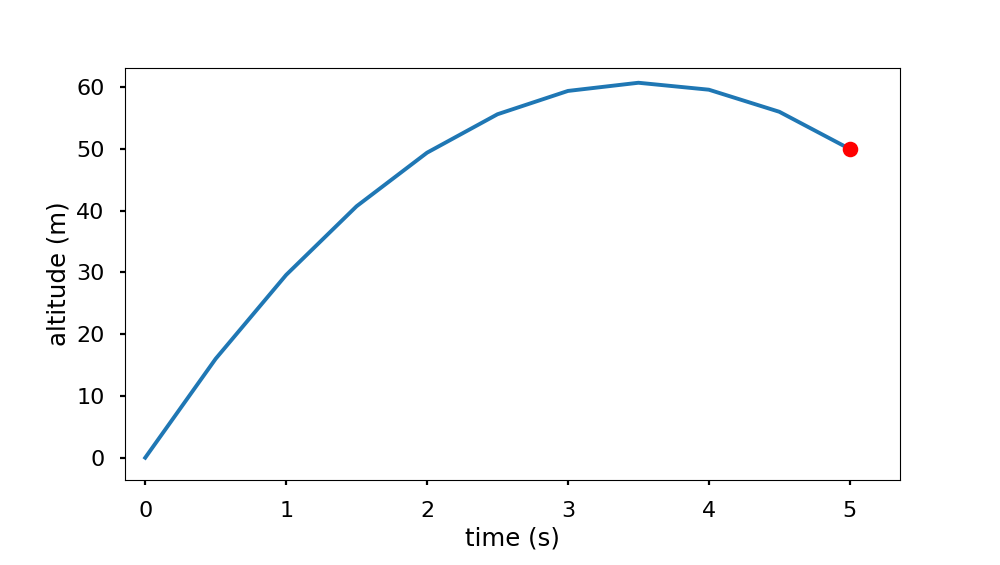
\includegraphics[width=0.9\textwidth]{figures/finite_difference}
	\caption{Example of linear regression for the determination of $\beta$.}
	\label{fig:finite_difference}
\end{figure} 

Now, let’s solve for $y'(0)$ in order to determine the intial velocity of the rocket. From the finite difference formula, we know that $\frac{dy}{dx}=\frac{y_{i+1}−y_{i−1}}{2h}$, which means that $y'(0)=\frac{y_1−y_{−1}}{2h}$, but we don’t know what is $y_{−1}$. Actually, we can calculate $y_{−1}$ since we know the $y$ values on each grid point. From the 2$^{nd}$ derivative finite difference formula, we know that $\frac{y_{−1}−2y_0+y_1}{h^2}=−g$, therefore, we can solve for $y_{−1}$ and then get the launching velocity. See the calculation below.

\begin{ipython}
y_n1 = -9.8*h**2 + 2*y[0] - y[1]
(y[1] - y_n1) / (2*h)
\end{ipython}
\begin{ioutput}
34.5
\end{ioutput}

% \section{Finite Differences in Option Pricing}
%The motivation behind the finite differencing is the application of the Black-Scholes Partial Differential Equation (PDE) framework (involving functions and their partial derivatives) whose price $S(t)$ is a function of
%$f(S,t)$, with $r$ as the risk-free rate, $t$ as the time to maturity, and $\sigma$ as the volatility of the underlying security:
%
%\begin{equation}
%rf = \cfrac{\partial f}{\partial t} + rS\cfrac{\partial f}{\partial S} + \cfrac{1}{2} \sigma^2 S^2 \cfrac{\partial ^2 f}{\partial t^2}
%\end{equation}
%
%The finite difference technique tends to converge faster than lattices and approximates complex exotic options very well.
%To solve a PDE by finite differences working backward in time, a discrete-time grid of size $M$ by $N$ is set up to reflect asset prices over a course of time, such that $S$ and
%$t$ take on the following values at each point on the grid:
%
%\begin{equation}
%\begin{gathered}
%S = 0, dS, 2dS, 3dS,\ldots, (M −1) dS, S_{max} \\
%t = 0, dt, 2dt, 3dt,\ldots (N −1) dt, T
%\end{gathered}
%\end{equation}
%
%It follows that by grid notation, $f_{i, j} = f (idS, jdt)$. $S_{max}$ is a suitably large asset price that cannot be reached by the maturity time, $T$. $dS$ and $dt$ are thus intervals between each node in the grid, incremented by price and time respectively. The terminal condition at expiration time $T$ for every value of $S$ is $\textrm{max}(S − K,0)$ for a call option with strike $K$ and $\textrm{max}(K − S,0)$ for a put option. The grid traverses backward from the terminal conditions, complying with the PDE while adhering to the boundary conditions of the grid, such as the payoff from an early exercise.
%
%The boundary conditions are defined values at the extreme ends of the nodes, where $i=0$ and $i=N$ for every time at $t$. Values at the boundaries are used to calculate the values of all other lattice nodes iteratively using the PDE.
%
%A visual representation of the grid is given by the following figure. As $i$ and $j$ increase from the top-left corner of the grid, the price $S$ tends toward $S_{max}$ (the maximum price possible) at the bottom-right corner of the grid:
%A number of ways to approximate the PDE are as follows: 
%
%\begin{itemize}
%\item Forward difference:
%\begin{equation}
%\cfrac{\partial f}{\partial S} = \cfrac{f_{i+1,j} − f_{i,j}}{\partial S},\quad \cfrac{\partial f}{\partial t} = \cfrac{f_{i,j+1} − f_{i,j}}{\partial t}
%\end{equation}
%
%\item Backward difference:
%\begin{equation}
%	\cfrac{\partial f}{\partial S} = \cfrac{f_{i,j} − f_{i-1,j}}{\partial S},\quad \cfrac{\partial f}{\partial t} = \cfrac{f_{i,j} − f_{i,j-1}}{\partial t}
%\end{equation}
%
%\item Central or symmetric difference:
%\begin{equation}
%	\cfrac{\partial f}{\partial S} = \cfrac{f_{i+1,j} − f_{i-1,j}}{2\partial S},\quad \cfrac{\partial f}{\partial t} = \cfrac{f_{i,j+1} − f_{i,j-1}}{2\partial t}
%\end{equation}
%
%\item The second derivative:
%\begin{equation}
%	\cfrac{\partial^2 f}{\partial S^2} = \cfrac{f_{i+1,j} − 2f_{i,j} +  f_{i-1,j}}{2\partial S^2}
%\end{equation}
%\end{itemize}
%
%Once we have the boundary conditions set up, we can now apply an iterative approach using the explicit, implicit, or Crank-Nicolson method.
%
%\subsection{The Explicit Method}
%The explicit method for approximating $f_{i, j}$ is given by:
%
%\begin{equation}
%rf_{i,j} = \cfrac{f_{i,j} − f_{i,j−1}}{dt} + ridS \cfrac{f_{i+1,j} − f_{i−1,j}}{2dS} +\cfrac{1}{2} \sigma^2 j^2 \cfrac{f_{i+1,j} + f_{i−1,j}}{dS^2}
%\end{equation}
%
%Here, it can be seen that the first difference is the backward difference with respect to $t$, the second difference is the central difference with respect to $S$, and the third difference is the second-order difference with respect to $S$. When we rearrange the terms, we have the following equation:
%
%\begin{equation}
%f_{i,j} =a^* f_{i-1,j+1} +b^* f_{i,j+1} +c^* f_{i+1,j+1}
%\end{equation}
%where $j=N−1,N−2,N−3,\ldots, 2,1,0$ and $i=1,2,3,\ldots, M−2,M−1$:
%
%\begin{equation}
%\begin{gathered}
%a^* = \cfrac{1}{2}dt(\sigma^2 i^2 −ri)\\
%b^* =1−dt(\sigma^2 i^2 −ri) \\
%c^* = \cfrac{1}{2}dt(\sigma^2 i^2 +ri)
%\end{gathered}	
%\end{equation} 
% 
%The iterative approach of the explicit method can be visually represented by the following figure:
%
%\begin{center}
%\begin{tikzpicture}
%	[parent anchor=east,child anchor=west,grow=east]
%	%\tikzstyle{every node}=[ball color=red,circle,text=white]
%	\tikzstyle{edge from parent}=[draw,ultra thick,red]
%	\node {$f_{i,j}$}
%	child {node {$f_{i+1,j+1}$}}
%	child {node {$f_{i,j+1}$}}
%	child {node {$f_{i-1,j+1}$}};
%\end{tikzpicture}
%\end{center}
%
%\subsection{\texttt{FiniteDifferences} class}
%As we will be writing the explicit, implicit, and Crank-Nicolson methods of finite differences in \texttt{python}, let's write a parent class that can inherit the common properties and functions of all three methods.
%
%We will create a class called \texttt{FiniteDifferences} that accepts and assigns all the required parameters in the constructor method.
%
%\begin{codebox}
%\begin{Verbatim}[commandchars=\\\{\}]
%\PY{k+kn}{import} \PY{n+nn}{numpy} \PY{k}{as} \PY{n+nn}{np}
%		
%\PY{k}{class} \PY{n+nc}{FiniteDifferences}\PY{p}{:}
%    \PY{k}{def} \PY{n+nf+fm}{\PYZus{}\PYZus{}init\PYZus{}\PYZus{}}\PY{p}{(}\PY{n+nb+bp}{self}\PY{p}{,} \PY{n}{S0}\PY{p}{,} \PY{n}{K}\PY{p}{,} \PY{n}{r}\PY{p}{,} \PY{n}{T}\PY{p}{,} \PY{n}{sigma}\PY{p}{,} \PY{n}{Smax}\PY{p}{,} \PY{n}{M}\PY{p}{,} \PY{n}{N}\PY{p}{,} \PY{n}{is\PYZus{}call} \PY{o}{=} \PY{k+kc}{True}\PY{p}{)}\PY{p}{:}
%        \PY{n+nb+bp}{self}\PY{o}{.}\PY{n}{S0} \PY{o}{=} \PY{n}{S0}
%        \PY{n+nb+bp}{self}\PY{o}{.}\PY{n}{K} \PY{o}{=} \PY{n}{K}
%        \PY{n+nb+bp}{self}\PY{o}{.}\PY{n}{r} \PY{o}{=} \PY{n}{r}
%        \PY{n+nb+bp}{self}\PY{o}{.}\PY{n}{T} \PY{o}{=} \PY{n}{T}
%        \PY{n+nb+bp}{self}\PY{o}{.}\PY{n}{sigma} \PY{o}{=} \PY{n}{sigma}
%        \PY{n+nb+bp}{self}\PY{o}{.}\PY{n}{Smax} \PY{o}{=} \PY{n}{Smax}
%        \PY{n+nb+bp}{self}\PY{o}{.}\PY{n}{M}\PY{p}{,} \PY{n+nb+bp}{self}\PY{o}{.}\PY{n}{N} \PY{o}{=} \PY{n+nb}{int}\PY{p}{(}\PY{n}{M}\PY{p}{)}\PY{p}{,} \PY{n+nb}{int}\PY{p}{(}\PY{n}{N}\PY{p}{)}
%        \PY{n+nb+bp}{self}\PY{o}{.}\PY{n}{is\PYZus{}call} \PY{o}{=} \PY{n}{is\PYZus{}call}
%        \PY{n+nb+bp}{self}\PY{o}{.}\PY{n}{dS} \PY{o}{=} \PY{n}{Smax} \PY{o}{/} \PY{n+nb}{float}\PY{p}{(}\PY{n+nb+bp}{self}\PY{o}{.}\PY{n}{M}\PY{p}{)}
%        \PY{n+nb+bp}{self}\PY{o}{.}\PY{n}{dt} \PY{o}{=} \PY{n}{T} \PY{o}{/} \PY{n+nb}{float}\PY{p}{(}\PY{n+nb+bp}{self}\PY{o}{.}\PY{n}{N}\PY{p}{)}
%        \PY{n+nb+bp}{self}\PY{o}{.}\PY{n}{i\PYZus{}values} \PY{o}{=} \PY{n}{np}\PY{o}{.}\PY{n}{arange}\PY{p}{(}\PY{n+nb+bp}{self}\PY{o}{.}\PY{n}{M}\PY{p}{)}
%        \PY{n+nb+bp}{self}\PY{o}{.}\PY{n}{j\PYZus{}values} \PY{o}{=} \PY{n}{np}\PY{o}{.}\PY{n}{arange}\PY{p}{(}\PY{n+nb+bp}{self}\PY{o}{.}\PY{n}{N}\PY{p}{)}
%        \PY{n+nb+bp}{self}\PY{o}{.}\PY{n}{grid} \PY{o}{=} \PY{n}{np}\PY{o}{.}\PY{n}{zeros}\PY{p}{(}\PY{n}{shape}\PY{o}{=}\PY{p}{(}\PY{n+nb+bp}{self}\PY{o}{.}\PY{n}{M}\PY{o}{+}\PY{l+m+mi}{1}\PY{p}{,} \PY{n+nb+bp}{self}\PY{o}{.}\PY{n}{N}\PY{o}{+}\PY{l+m+mi}{1}\PY{p}{)}\PY{p}{)} 
%        \PY{n+nb+bp}{self}\PY{o}{.}\PY{n}{boundary\PYZus{}conds} \PY{o}{=} \PY{n}{np}\PY{o}{.}\PY{n}{linspace}\PY{p}{(}\PY{l+m+mi}{0}\PY{p}{,} \PY{n}{Smax}\PY{p}{,} \PY{n+nb+bp}{self}\PY{o}{.}\PY{n}{M}\PY{o}{+}\PY{l+m+mi}{1}\PY{p}{)}
%		
%    \PY{k}{def} \PY{n+nf}{\PYZus{}setup\PYZus{}boundary\PYZus{}conditions\PYZus{}}\PY{p}{(}\PY{n+nb+bp}{self}\PY{p}{)}\PY{p}{:}
%        \PY{k}{pass}
%		
%    \PY{k}{def} \PY{n+nf}{\PYZus{}setup\PYZus{}coefficients\PYZus{}}\PY{p}{(}\PY{n+nb+bp}{self}\PY{p}{)}\PY{p}{:}
%        \PY{k}{pass}
%		
%    \PY{k}{def} \PY{n+nf}{\PYZus{}traverse\PYZus{}grid\PYZus{}}\PY{p}{(}\PY{n+nb+bp}{self}\PY{p}{)}\PY{p}{:}
%        \PY{k}{pass}
%		
%    \PY{k}{def} \PY{n+nf}{\PYZus{}interpolate\PYZus{}}\PY{p}{(}\PY{n+nb+bp}{self}\PY{p}{)}\PY{p}{:}
%        \PY{k}{return} \PY{n}{np}\PY{o}{.}\PY{n}{interp}\PY{p}{(}\PY{n+nb+bp}{self}\PY{o}{.}\PY{n}{S0}\PY{p}{,} \PY{n+nb+bp}{self}\PY{o}{.}\PY{n}{boundary\PYZus{}conds}\PY{p}{,} \PY{n+nb+bp}{self}\PY{o}{.}\PY{n}{grid}\PY{p}{[}\PY{p}{:}\PY{p}{,} \PY{l+m+mi}{0}\PY{p}{]}\PY{p}{)}
%		
%    \PY{k}{def} \PY{n+nf}{price}\PY{p}{(}\PY{n+nb+bp}{self}\PY{p}{)}\PY{p}{:} 
%        \PY{n+nb+bp}{self}\PY{o}{.}\PY{n}{\PYZus{}setup\PYZus{}boundary\PYZus{}conditions\PYZus{}}\PY{p}{(}\PY{p}{)} 
%        \PY{n+nb+bp}{self}\PY{o}{.}\PY{n}{\PYZus{}setup\PYZus{}coefficients\PYZus{}}\PY{p}{(}\PY{p}{)} 
%        \PY{n+nb+bp}{self}\PY{o}{.}\PY{n}{\PYZus{}traverse\PYZus{}grid\PYZus{}}\PY{p}{(}\PY{p}{)}
%        \PY{k}{return} \PY{n+nb+bp}{self}\PY{o}{.}\PY{n}{\PYZus{}interpolate\PYZus{}}\PY{p}{(}\PY{p}{)}
%\end{Verbatim}
%\end{codebox}
%
%All of these methods are protected methods and may be overwritten by derived classes. The pass keyword simply does nothing; the derived classes will provide specific implementations of these functions.
%
%\subsubsection{\texttt{FDExplicitEu} class}
%
%The \texttt{python} implementation of finite differences by the explicit method is given in the following \texttt{FDExplicitEu} class, which inherits from the \texttt{FiniteDifferences} class and overrides the required implementation methods.
%
%\begin{codebox}
%\begin{Verbatim}[commandchars=\\\{\}]
%\PY{k+kn}{import} \PY{n+nn}{numpy} \PY{k}{as} \PY{n+nn}{np}
%		
%\PY{k}{class} \PY{n+nc}{FDExplicitEu}\PY{p}{(}\PY{n}{FiniteDifferences}\PY{p}{)}\PY{p}{:}
%    \PY{k}{def} \PY{n+nf}{\PYZus{}setup\PYZus{}boundary\PYZus{}conditions\PYZus{}}\PY{p}{(}\PY{n+nb+bp}{self}\PY{p}{)}\PY{p}{:} 
%        \PY{k}{if} \PY{n+nb+bp}{self}\PY{o}{.}\PY{n}{is\PYZus{}call}\PY{p}{:}
%            \PY{n+nb+bp}{self}\PY{o}{.}\PY{n}{grid}\PY{p}{[}\PY{p}{:}\PY{p}{,} \PY{o}{\PYZhy{}}\PY{l+m+mi}{1}\PY{p}{]} \PY{o}{=} \PY{n}{np}\PY{o}{.}\PY{n}{maximum}\PY{p}{(}\PY{n+nb+bp}{self}\PY{o}{.}\PY{n}{boundary\PYZus{}conds} \PY{o}{\PYZhy{}} \PY{n+nb+bp}{self}\PY{o}{.}\PY{n}{K}\PY{p}{,} \PY{l+m+mi}{0}\PY{p}{)}
%            \PY{n+nb+bp}{self}\PY{o}{.}\PY{n}{grid}\PY{p}{[}\PY{o}{\PYZhy{}}\PY{l+m+mi}{1}\PY{p}{,} \PY{p}{:}\PY{o}{\PYZhy{}}\PY{l+m+mi}{1}\PY{p}{]} \PY{o}{=} \PY{p}{(}\PY{n+nb+bp}{self}\PY{o}{.}\PY{n}{Smax} \PY{o}{\PYZhy{}} \PY{n+nb+bp}{self}\PY{o}{.}\PY{n}{K}\PY{p}{)} \PY{o}{*} 
%                \PY{n}{np}\PY{o}{.}\PY{n}{exp}\PY{p}{(}\PY{o}{\PYZhy{}}\PY{n+nb+bp}{self}\PY{o}{.}\PY{n}{r} \PY{o}{*} \PY{n+nb+bp}{self}\PY{o}{.}\PY{n}{dt} \PY{o}{*} \PY{p}{(}\PY{n+nb+bp}{self}\PY{o}{.}\PY{n}{N}\PY{o}{\PYZhy{}}\PY{n+nb+bp}{self}\PY{o}{.}\PY{n}{j\PYZus{}values}\PY{p}{)}\PY{p}{)}
%        \PY{k}{else}\PY{p}{:}
%            \PY{n+nb+bp}{self}\PY{o}{.}\PY{n}{grid}\PY{p}{[}\PY{p}{:}\PY{p}{,} \PY{o}{\PYZhy{}}\PY{l+m+mi}{1}\PY{p}{]} \PY{o}{=} \PY{n}{np}\PY{o}{.}\PY{n}{maximum}\PY{p}{(}\PY{n+nb+bp}{self}\PY{o}{.}\PY{n}{K}\PY{o}{\PYZhy{}}\PY{n+nb+bp}{self}\PY{o}{.}\PY{n}{boundary\PYZus{}conds}\PY{p}{,} \PY{l+m+mi}{0}\PY{p}{)} 
%            \PY{n+nb+bp}{self}\PY{o}{.}\PY{n}{grid}\PY{p}{[}\PY{l+m+mi}{0}\PY{p}{,} \PY{p}{:}\PY{o}{\PYZhy{}}\PY{l+m+mi}{1}\PY{p}{]} \PY{o}{=} \PY{p}{(}\PY{n+nb+bp}{self}\PY{o}{.}\PY{n}{K} \PY{o}{\PYZhy{}} \PY{n+nb+bp}{self}\PY{o}{.}\PY{n}{Smax}\PY{p}{)} \PY{o}{*} \PY{n}{np}\PY{o}{.}\PY{n}{exp}\PY{p}{(}\PY{o}{\PYZhy{}}\PY{n+nb+bp}{self}\PY{o}{.}\PY{n}{r} 
%                \PY{o}{*} \PY{n+nb+bp}{self}\PY{o}{.}\PY{n}{dt} \PY{o}{*} \PY{p}{(}\PY{n+nb+bp}{self}\PY{o}{.}\PY{n}{N}\PY{o}{\PYZhy{}}\PY{n+nb+bp}{self}\PY{o}{.}\PY{n}{j\PYZus{}values}\PY{p}{)}\PY{p}{)}
%		
%    \PY{k}{def} \PY{n+nf}{\PYZus{}setup\PYZus{}coefficients\PYZus{}}\PY{p}{(}\PY{n+nb+bp}{self}\PY{p}{)}\PY{p}{:}
%        \PY{n+nb+bp}{self}\PY{o}{.}\PY{n}{a} \PY{o}{=} \PY{l+m+mf}{0.5}\PY{o}{*}\PY{n+nb+bp}{self}\PY{o}{.}\PY{n}{dt}\PY{o}{*}\PY{p}{(}\PY{p}{(}\PY{n+nb+bp}{self}\PY{o}{.}\PY{n}{sigma}\PY{o}{*}\PY{o}{*}\PY{l+m+mi}{2}\PY{p}{)} \PY{o}{*} \PY{p}{(}\PY{n+nb+bp}{self}\PY{o}{.}\PY{n}{i\PYZus{}values}\PY{o}{*}\PY{o}{*}\PY{l+m+mi}{2}\PY{p}{)} 
%                 \PY{o}{\PYZhy{}} \PY{n+nb+bp}{self}\PY{o}{.}\PY{n}{r}\PY{o}{*}\PY{n+nb+bp}{self}\PY{o}{.}\PY{n}{i\PYZus{}values}\PY{p}{)} 
%        \PY{n+nb+bp}{self}\PY{o}{.}\PY{n}{b} \PY{o}{=} \PY{l+m+mi}{1} \PY{o}{\PYZhy{}} \PY{n+nb+bp}{self}\PY{o}{.}\PY{n}{dt}\PY{o}{*}\PY{p}{(}\PY{p}{(}\PY{n+nb+bp}{self}\PY{o}{.}\PY{n}{sigma}\PY{o}{*}\PY{o}{*}\PY{l+m+mi}{2}\PY{p}{)} \PY{o}{*} \PY{p}{(}\PY{n+nb+bp}{self}\PY{o}{.}\PY{n}{i\PYZus{}values}\PY{o}{*}\PY{o}{*}\PY{l+m+mi}{2}\PY{p}{)} 
%                 \PY{o}{+} \PY{n+nb+bp}{self}\PY{o}{.}\PY{n}{r}\PY{p}{)}
%        \PY{n+nb+bp}{self}\PY{o}{.}\PY{n}{c} \PY{o}{=} \PY{l+m+mf}{0.5}\PY{o}{*}\PY{n+nb+bp}{self}\PY{o}{.}\PY{n}{dt}\PY{o}{*}\PY{p}{(}\PY{p}{(}\PY{n+nb+bp}{self}\PY{o}{.}\PY{n}{sigma}\PY{o}{*}\PY{o}{*}\PY{l+m+mi}{2}\PY{p}{)} \PY{o}{*} \PY{p}{(}\PY{n+nb+bp}{self}\PY{o}{.}\PY{n}{i\PYZus{}values}\PY{o}{*}\PY{o}{*}\PY{l+m+mi}{2}\PY{p}{)} 
%                 \PY{o}{+} \PY{n+nb+bp}{self}\PY{o}{.}\PY{n}{r}\PY{o}{*}\PY{n+nb+bp}{self}\PY{o}{.}\PY{n}{i\PYZus{}values}\PY{p}{)}
%		
%    \PY{k}{def} \PY{n+nf}{\PYZus{}traverse\PYZus{}grid\PYZus{}}\PY{p}{(}\PY{n+nb+bp}{self}\PY{p}{)}\PY{p}{:}
%        \PY{k}{for} \PY{n}{j} \PY{o+ow}{in} \PY{n+nb}{reversed}\PY{p}{(}\PY{n+nb+bp}{self}\PY{o}{.}\PY{n}{j\PYZus{}values}\PY{p}{)}\PY{p}{:}
%            \PY{k}{for} \PY{n}{i} \PY{o+ow}{in} \PY{n+nb}{range}\PY{p}{(}\PY{n+nb+bp}{self}\PY{o}{.}\PY{n}{M}\PY{p}{)}\PY{p}{[}\PY{l+m+mi}{2}\PY{p}{:}\PY{p}{]}\PY{p}{:}
%                \PY{n+nb+bp}{self}\PY{o}{.}\PY{n}{grid}\PY{p}{[}\PY{n}{i}\PY{p}{,}\PY{n}{j}\PY{p}{]} \PY{o}{=} \PY{n+nb+bp}{self}\PY{o}{.}\PY{n}{a}\PY{p}{[}\PY{n}{i}\PY{p}{]}\PY{o}{*}\PY{n+nb+bp}{self}\PY{o}{.}\PY{n}{grid}\PY{p}{[}\PY{n}{i}\PY{o}{\PYZhy{}}\PY{l+m+mi}{1}\PY{p}{,}\PY{n}{j}\PY{o}{+}\PY{l+m+mi}{1}\PY{p}{]} \PY{o}{+} 
%                                 \PY{n+nb+bp}{self}\PY{o}{.}\PY{n}{b}\PY{p}{[}\PY{n}{i}\PY{p}{]}\PY{o}{*}\PY{n+nb+bp}{self}\PY{o}{.}\PY{n}{grid}\PY{p}{[}\PY{n}{i}\PY{p}{,}\PY{n}{j}\PY{o}{+}\PY{l+m+mi}{1}\PY{p}{]} \PY{o}{+} 
%                                 \PY{n+nb+bp}{self}\PY{o}{.}\PY{n}{c}\PY{p}{[}\PY{n}{i}\PY{p}{]}\PY{o}{*}\PY{n+nb+bp}{self}\PY{o}{.}\PY{n}{grid}\PY{p}{[}\PY{n}{i}\PY{o}{+}\PY{l+m+mi}{1}\PY{p}{,}\PY{n}{j}\PY{o}{+}\PY{l+m+mi}{1}\PY{p}{]}
%\end{Verbatim}
%\end{codebox}
%
%On completion of traversing the grid structure, the first column contains the present value of the initial asset prices at t=0. The \texttt{interp} function of \texttt{numpy} is used to perform a linear interpolation to approximate the option value.
%
%Besides using linear interpolation as the most common choice for the interpolation method, the other methods such as the spline or cubic may be used to approximate the option value.
%Consider the example of an European put option. The underlying stock price is \$50 with a volatility of 0.4. The strike price of the put option is \$50 with an expiration time of 5 months. The risk-free rate is 10 percent.
%We can price the option using the explicit method with a $S_{max}$ value of 100, an M value of 1000, and a N 
%
%\begin{codebox}
%\begin{Verbatim}[commandchars=\\\{\}]
%\PY{n}{option} \PY{o}{=} \PY{n}{FDExplicitEu}\PY{p}{(}\PY{l+m+mi}{50}\PY{p}{,} \PY{l+m+mi}{50}\PY{p}{,} \PY{l+m+mf}{0.1}\PY{p}{,} \PY{l+m+mf}{5.}\PY{o}{/}\PY{l+m+mf}{12.}\PY{p}{,} \PY{l+m+mf}{0.4}\PY{p}{,} \PY{l+m+mi}{100}\PY{p}{,} \PY{l+m+mi}{100}\PY{p}{,} \PY{l+m+mi}{1000}\PY{p}{,} \PY{k+kc}{False}\PY{p}{)}
%\PY{n+nb}{print} \PY{p}{(}\PY{n}{option}\PY{o}{.}\PY{n}{price}\PY{p}{(}\PY{p}{)}\PY{p}{)}
%
%4.072882278148043
%\end{Verbatim}
%\end{codebox}
%
%What happens when other values of M and N are chosen improperly?
%
%\begin{codebox}
%\begin{Verbatim}[commandchars=\\\{\}]
%\PY{n}{option} \PY{o}{=} \PY{n}{FDExplicitEu}\PY{p}{(}\PY{l+m+mi}{50}\PY{p}{,} \PY{l+m+mi}{50}\PY{p}{,} \PY{l+m+mf}{0.1}\PY{p}{,} \PY{l+m+mf}{5.}\PY{o}{/}\PY{l+m+mf}{12.}\PY{p}{,} \PY{l+m+mf}{0.4}\PY{p}{,} \PY{l+m+mi}{100}\PY{p}{,} \PY{l+m+mi}{100}\PY{p}{,} \PY{l+m+mi}{100}\PY{p}{,} \PY{k+kc}{False}\PY{p}{)}
%\PY{n+nb}{print} \PY{p}{(}\PY{n}{option}\PY{o}{.}\PY{n}{price}\PY{p}{(}\PY{p}{)}\PY{p}{)}
%
%-1.6291077072251005e+53
%\end{Verbatim}
%\end{codebox}
%
%It appears that the explicit method of the finite difference scheme suffers from instability problems.
%
%\subsubsection{\texttt{FDImplicitEu} class}
%
%The instability problem of the explicit method can be overcome using the forward difference with respect to time. The implicit method for approximating $f_{i, j}$ is given by:
%
%\begin{equation}
%	rf_{i,j} = \cfrac{f_{i,j} − f_{i,j−1}}{dt} + ridS \cfrac{f_{i+1,j} − f_{i−1,j}}{2dS} +\cfrac{1}{2} \sigma^2 j^2 \cfrac{f_{i+1,j} + f_{i−1,j}}{dS^2}
%\end{equation}
%
%Here, it can be seen that the only difference between the implicit and explicit approximating scheme lies in the first difference, where the forward difference with respect to $t$ is used in the implicit scheme. When we rearrange the terms, we have the following expression:
%
%\begin{equation}
%	f_{i,j+1} = a_i f_{i-1,j} +b_i f_{i,j} +c_i f_{i+1,j}
%\end{equation}
%where $j=N−1,N−2,N−3,\ldots, 2,1,0$ and $i=1,2,3,\ldots, M−1$:
%
%\begin{equation}
%	\begin{gathered}
%		a_i = \cfrac{1}{2}dt(ri-\sigma^2 i^2)\\
%		b_i =1+dt(ri+\sigma^2 i^2) \\
%		c_i = -\cfrac{1}{2}+dt(\sigma^2 i^2 + ri)
%	\end{gathered}	
%\end{equation} 
%
%The iterative approach of the explicit method can be visually represented by the following figure:
%
%\begin{center}
%	\begin{tikzpicture}
%		[parent anchor=east,child anchor=west,grow=east]
%		%\tikzstyle{every node}=[ball color=red,circle,text=white]
%		\tikzstyle{edge from parent}=[draw,ultra thick,red]
%		\node {$f_{i+1,j}$}
%		 node {$f_{i,j}$}
%			child {node {$f_{i,j+1}$}}
%		 node {$f_{i-1,j}$};
%	\end{tikzpicture}
%\end{center}
%
%From the figure, it is intuitive to note that values of $j + 1$ are required to be computed before they can be used in the next iterative step, as the grid traverses backward.
%In the implicit scheme, the grid can be thought of as representing a system of linear equations at each iteration, as follows:
%
%\begin{equation*}
%\begin{bmatrix}
%b_1    & c_1 & 0   & \cdots & 0 & 0 \\
%a_2    & b_2 & c_2 & \cdots & 0 & 0 \\
%0      & 0   & b_3 & \cdots & 0 & 0 \\
%\vdots & \vdots & \vdots & \ddots & \vdots & \vdots \\
%0   & 0 & 0 & a_{M-2} & b_{M-2} & c_{M-2} \\
%0   & 0 & 0 & \cdots & a_{M-1} & b_{M-1}
%\end{bmatrix}
%\begin{bmatrix} 
%	f_{1,j}\\
%	f_{2,j}\\
%	f_{3,j}\\
%	\vdots\\
%	f_{M-2,j}\\
%	f_{M-1,j}\\
%\end{bmatrix} +
%\begin{bmatrix}
%a_1 f_{0,j}\\
%0\\
%0\\
%\vdots\\
%0\\
%c_{M-1}f_{M,j}\\
%\end{bmatrix} =
%\begin{bmatrix} 
%f_{1,j+1}\\
%f_{2,j+1}\\
%f_{3,j+1}\\
%\vdots\\
%f_{M-2,j+1}\\
%f_{M-1,j+1}\\
%\end{bmatrix}
%\end{equation*}
%\noindent
%By rearranging the terms, we get the following equation:
%\begin{equation*}
%\begin{bmatrix}
%b_1    & c_1 & 0   & \cdots & 0 & 0 \\
%a_2    & b_2 & c_2 & \cdots & 0 & 0 \\
%0      & 0   & b_3 & \cdots & 0 & 0 \\
%\vdots & \vdots & \vdots & \ddots & \vdots & \vdots \\
%0   & 0 & 0 & a_{M-2} & b_{M-2} & c_{M-2} \\
%0   & 0 & 0 & \cdots & a_{M-1} & b_{M-1}
%\end{bmatrix}
%\begin{bmatrix}
%f_{1,j}\\
%f_{2,j}\\
%f_{3,j}\\
%\vdots\\
%f_{M-2,j}\\
%f_{M-1,j}
%\end{bmatrix} = 
%\begin{bmatrix}
%f_{1,j+1}\\
%f_{2,j+1}\\
%f_{3,j+1}\\
%\vdots\\
%f_{M-2,j+1}\\
%f_{M-1,j+1}
%\end{bmatrix} - 
%\begin{bmatrix}
%a_1 f_{0,j}\\
%0\\
%0\\
%\vdots\\
%0\\
%c_{M-1}f_{M,j}
%\end{bmatrix}
%\end{equation*}
%
%The linear system of equations can be represented in the form of $[A]x = [B]$, where we want to solve for values of $x$ in each iteration. Since the matrix $[A]$ is tri-diagonal, we can use the LU factorization, where $[A]=[L][U]$, for faster computation. 
%
%The \texttt{python} implementation of the implicit scheme is given in the following \texttt{FDImplicitEu} class. We can inherit the implementation of the explicit method from the \texttt{FDExplicitEu} class discussed earlier and override the necessary methods of interest:
%
%\begin{codebox}
%\begin{Verbatim}[commandchars=\\\{\}]
%\PY{k+kn}{import} \PY{n+nn}{scipy}\PY{n+nn}{.}\PY{n+nn}{linalg} \PY{k}{as} \PY{n+nn}{linalg}
%		
%\PY{k}{class} \PY{n+nc}{FDImplicitEu}\PY{p}{(}\PY{n}{FDExplicitEu}\PY{p}{)}\PY{p}{:}
%    \PY{k}{def} \PY{n+nf}{\PYZus{}setup\PYZus{}coefficients\PYZus{}}\PY{p}{(}\PY{n+nb+bp}{self}\PY{p}{)}\PY{p}{:}
%        \PY{n+nb+bp}{self}\PY{o}{.}\PY{n}{a} \PY{o}{=} \PY{l+m+mf}{0.5}\PY{o}{*}\PY{p}{(}\PY{n+nb+bp}{self}\PY{o}{.}\PY{n}{r}\PY{o}{*}\PY{n+nb+bp}{self}\PY{o}{.}\PY{n}{dt}\PY{o}{*}\PY{n+nb+bp}{self}\PY{o}{.}\PY{n}{i\PYZus{}values} \PY{o}{\PYZhy{}} \PY{p}{(}\PY{n+nb+bp}{self}\PY{o}{.}\PY{n}{sigma}\PY{o}{*}\PY{o}{*}\PY{l+m+mi}{2}\PY{p}{)}\PY{o}{*}\PY{n+nb+bp}{self}\PY{o}{.}\PY{n}{dt}\PY{o}{*}\PY{p}{(}\PY{n+nb+bp}{self}\PY{o}{.}\PY{n}{i\PYZus{}values}\PY{o}{*}\PY{o}{*}\PY{l+m+mi}{2}\PY{p}{)}\PY{p}{)} 
%        \PY{n+nb+bp}{self}\PY{o}{.}\PY{n}{b} \PY{o}{=} \PY{l+m+mi}{1} \PY{o}{+} \PY{p}{(}\PY{n+nb+bp}{self}\PY{o}{.}\PY{n}{sigma}\PY{o}{*}\PY{o}{*}\PY{l+m+mi}{2}\PY{p}{)}\PY{o}{*}\PY{n+nb+bp}{self}\PY{o}{.}\PY{n}{dt}\PY{o}{*}\PY{p}{(}\PY{n+nb+bp}{self}\PY{o}{.}\PY{n}{i\PYZus{}values}\PY{o}{*}\PY{o}{*}\PY{l+m+mi}{2}\PY{p}{)} \PY{o}{+} \PY{n+nb+bp}{self}\PY{o}{.}\PY{n}{r}\PY{o}{*}\PY{n+nb+bp}{self}\PY{o}{.}\PY{n}{dt} 
%        \PY{n+nb+bp}{self}\PY{o}{.}\PY{n}{c} \PY{o}{=} \PY{o}{\PYZhy{}}\PY{l+m+mf}{0.5}\PY{o}{*}\PY{p}{(}\PY{n+nb+bp}{self}\PY{o}{.}\PY{n}{r} \PY{o}{*} \PY{n+nb+bp}{self}\PY{o}{.}\PY{n}{dt}\PY{o}{*}\PY{n+nb+bp}{self}\PY{o}{.}\PY{n}{i\PYZus{}values} \PY{o}{+} \PY{p}{(}\PY{n+nb+bp}{self}\PY{o}{.}\PY{n}{sigma}\PY{o}{*}\PY{o}{*}\PY{l+m+mi}{2}\PY{p}{)}\PY{o}{*}\PY{n+nb+bp}{self}\PY{o}{.}\PY{n}{dt}\PY{o}{*}\PY{p}{(}\PY{n+nb+bp}{self}\PY{o}{.}\PY{n}{i\PYZus{}values}\PY{o}{*}\PY{o}{*}\PY{l+m+mi}{2}\PY{p}{)}\PY{p}{)} 
%        \PY{n+nb+bp}{self}\PY{o}{.}\PY{n}{coeffs} \PY{o}{=} \PY{n}{np}\PY{o}{.}\PY{n}{diag}\PY{p}{(}\PY{n+nb+bp}{self}\PY{o}{.}\PY{n}{a}\PY{p}{[}\PY{l+m+mi}{2}\PY{p}{:}\PY{n+nb+bp}{self}\PY{o}{.}\PY{n}{M}\PY{p}{]}\PY{p}{,} \PY{o}{\PYZhy{}}\PY{l+m+mi}{1}\PY{p}{)} \PY{o}{+} \PY{n}{np}\PY{o}{.}\PY{n}{diag}\PY{p}{(}\PY{n+nb+bp}{self}\PY{o}{.}\PY{n}{b}\PY{p}{[}\PY{l+m+mi}{1}\PY{p}{:}\PY{n+nb+bp}{self}\PY{o}{.}\PY{n}{M}\PY{p}{]}\PY{p}{)} \PY{o}{+} \PY{n}{np}\PY{o}{.}\PY{n}{diag}\PY{p}{(}\PY{n+nb+bp}{self}\PY{o}{.}\PY{n}{c}\PY{p}{[}\PY{l+m+mi}{1}\PY{p}{:}\PY{n+nb+bp}{self}\PY{o}{.}\PY{n}{M}\PY{o}{\PYZhy{}}\PY{l+m+mi}{1}\PY{p}{]}\PY{p}{,} \PY{l+m+mi}{1}\PY{p}{)}
%		
%    \PY{k}{def} \PY{n+nf}{\PYZus{}traverse\PYZus{}grid\PYZus{}}\PY{p}{(}\PY{n+nb+bp}{self}\PY{p}{)}\PY{p}{:}
%        \PY{n}{P}\PY{p}{,} \PY{n}{L}\PY{p}{,} \PY{n}{U} \PY{o}{=} \PY{n}{linalg}\PY{o}{.}\PY{n}{lu}\PY{p}{(}\PY{n+nb+bp}{self}\PY{o}{.}\PY{n}{coeffs}\PY{p}{)}
%        \PY{n}{aux} \PY{o}{=} \PY{n}{np}\PY{o}{.}\PY{n}{zeros}\PY{p}{(}\PY{n+nb+bp}{self}\PY{o}{.}\PY{n}{M}\PY{o}{\PYZhy{}}\PY{l+m+mi}{1}\PY{p}{)}
%        \PY{k}{for} \PY{n}{j} \PY{o+ow}{in} \PY{n+nb}{reversed}\PY{p}{(}\PY{n+nb}{range}\PY{p}{(}\PY{n+nb+bp}{self}\PY{o}{.}\PY{n}{N}\PY{p}{)}\PY{p}{)}\PY{p}{:}
%            \PY{n}{aux}\PY{p}{[}\PY{l+m+mi}{0}\PY{p}{]} \PY{o}{=} \PY{n}{np}\PY{o}{.}\PY{n}{dot}\PY{p}{(}\PY{o}{\PYZhy{}}\PY{n+nb+bp}{self}\PY{o}{.}\PY{n}{a}\PY{p}{[}\PY{l+m+mi}{1}\PY{p}{]}\PY{p}{,} \PY{n+nb+bp}{self}\PY{o}{.}\PY{n}{grid}\PY{p}{[}\PY{l+m+mi}{0}\PY{p}{,} \PY{n}{j}\PY{p}{]}\PY{p}{)}
%            \PY{n}{x1} \PY{o}{=} \PY{n}{linalg}\PY{o}{.}\PY{n}{solve}\PY{p}{(}\PY{n}{L}\PY{p}{,} \PY{n+nb+bp}{self}\PY{o}{.}\PY{n}{grid}\PY{p}{[}\PY{l+m+mi}{1}\PY{p}{:}\PY{n+nb+bp}{self}\PY{o}{.}\PY{n}{M}\PY{p}{,} \PY{n}{j}\PY{o}{+}\PY{l+m+mi}{1}\PY{p}{]}\PY{o}{+}\PY{n}{aux}\PY{p}{)} 
%            \PY{n}{x2} \PY{o}{=} \PY{n}{linalg}\PY{o}{.}\PY{n}{solve}\PY{p}{(}\PY{n}{U}\PY{p}{,} \PY{n}{x1}\PY{p}{)}
%            \PY{n+nb+bp}{self}\PY{o}{.}\PY{n}{grid}\PY{p}{[}\PY{l+m+mi}{1}\PY{p}{:}\PY{n+nb+bp}{self}\PY{o}{.}\PY{n}{M}\PY{p}{,} \PY{n}{j}\PY{p}{]} \PY{o}{=} \PY{n}{x2}
%\end{Verbatim}
%\end{codebox}
%
%Using the same example as with the explicit scheme, we can price an European put option using the implicit scheme:
%
%\begin{codebox}
%\begin{Verbatim}[commandchars=\\\{\}]
%\PY{n}{option} \PY{o}{=} \PY{n}{FDImplicitEu}\PY{p}{(}\PY{l+m+mi}{50}\PY{p}{,} \PY{l+m+mi}{50}\PY{p}{,} \PY{l+m+mf}{0.1}\PY{p}{,} \PY{l+m+mf}{5.}\PY{o}{/}\PY{l+m+mf}{12.}\PY{p}{,} \PY{l+m+mf}{0.4}\PY{p}{,} \PY{l+m+mi}{100}\PY{p}{,} \PY{l+m+mi}{100}\PY{p}{,} \PY{l+m+mi}{100}\PY{p}{,} \PY{k+kc}{False}\PY{p}{)}
%\PY{n+nb}{print} \PY{p}{(}\PY{n}{option}\PY{o}{.}\PY{n}{price}\PY{p}{(}\PY{p}{)}\PY{p}{)}
%
%4.065801939431454
%
%\PY{n}{option} \PY{o}{=} \PY{n}{FDImplicitEu}\PY{p}{(}\PY{l+m+mi}{50}\PY{p}{,} \PY{l+m+mi}{50}\PY{p}{,} \PY{l+m+mf}{0.1}\PY{p}{,} \PY{l+m+mf}{5.}\PY{o}{/}\PY{l+m+mf}{12.}\PY{p}{,} \PY{l+m+mf}{0.4}\PY{p}{,} \PY{l+m+mi}{100}\PY{p}{,} \PY{l+m+mi}{100}\PY{p}{,} \PY{l+m+mi}{1000}\PY{p}{,} \PY{k+kc}{False}\PY{p}{)}
%\PY{n+nb}{print} \PY{p}{(}\PY{n}{option}\PY{o}{.}\PY{n}{price}\PY{p}{(}\PY{p}{)}\PY{p}{)}
%
%4.071594188049893
%\end{Verbatim}
%\end{codebox}
%
%Given the current parameters and input data, it is observed that there are no stability issues with the implicit scheme.
%
%\subsubsection{The Crank-Nicolson Method}
%Another way of avoiding the instability issue, as seen in the explicit method, is to use the Crank-Nicolson method. The Crank-Nicolson method converges much more quickly using a combination of the explicit and implicit methods, taking the average of both. This leads us to the following equation:
%
%
%%1rfi,j−1 +1rfi,j 22
%%fi,j − fi,j−1 1  fi+1,j−1 − fi−1,j−1  1  fi+1,j − fi−1,j  = dt 2 ridS  2dS  + 2 ridS  2dS  
%%        +1σ2i2dS2  fi+1,j−1 −2fi,j−1 + fi−1,j−1  4  dS2 
%%   +1σ2i2dS2fi+1,j −2fi,j +fi−1,j 
%%4  dS2  
%%  This equation can also be rewritten as follows:
%%−αi fi−1, j−1 +(1−βi ) fi, j−1 −γi fi+1, j−1 =αi fi−1, j +(1−βi ) fi, j−1 −γi fi+1, j Here:
%
%\begin{equation}
%\begin{gathered}
%\alpha_i = \cfrac{dt}{4}(\sigma^2 i^2 − ri)\\
%\beta_i  = \cfrac{dt}{2}(\sigma^2 i^2 + ri)\\
%\gamma_i = \cfrac{dt}{4}(\sigma^2 i^2 + ri) 
%\end{gathered}
%\end{equation}
%
%The iterative approach of the implicit scheme can be visually represented by the following figure:
%
%\begin{center}
%	\begin{tikzpicture}
%		[parent anchor=east,child anchor=west,grow=east]
%		%\tikzstyle{every node}=[ball color=red,circle,text=white]
%		\tikzstyle{edge from parent}=[draw,ultra thick,red]
%		\node {$f_{i+1,j}$}
%		node {$f_{i,j}$}
%		child {node {$f_{i,j+1}$}}
%		node {$f_{i-1,j}$};
%	\end{tikzpicture}
%\end{center}
%
%We can treat the equations as a system of linear equations in a matrix form:
%%  Here:
%%M1 fj−1 =M2 fj
%%1−β1 −γ1 0 0 0 0 
%%−α1−β−γ 0 0 0 222
%%0−α31−β3−γ3 00 M1=0 0 􏰦 􏰦 􏰦 0
%%
%%0 0 0 −αM−2 1−βM−2 −γM−2 
%%0 0 0 0 −α 1−β  M−1 M−1
%%1+β1 γ1 0 0 0 0 α1+βγ 0 0 0
%%222
%%0α31+β3−γ3 00 M2=0 0􏰦􏰦􏰦 0
%%
%%0 0 0 αM−2 1+βM−2 γM−2  
%%0 0 0 0 α 1+β  M−1 M−1
%%We can solve for the matrix M on every iterative procedure. [ 109 ]
%%f=f ,f ,...,f T i  1,j 2,j M1−1,j
%
%\subsubsection{\texttt{FDCnEu} class}
%The \texttt{python} implementation of the Crank-Nicolson method is given in the following \texttt{FDCnEu} class, which inherits from the \texttt{FDExplicitEu} class and overrides the usual methods.
%
%\begin{codebox}
%\begin{Verbatim}[commandchars=\\\{\}]
%\PY{k}{class} \PY{n+nc}{FDCnEu}\PY{p}{(}\PY{n}{FDExplicitEu}\PY{p}{)}\PY{p}{:}
%    \PY{k}{def} \PY{n+nf}{\PYZus{}setup\PYZus{}coefficients\PYZus{}}\PY{p}{(}\PY{n+nb+bp}{self}\PY{p}{)}\PY{p}{:} 
%        \PY{n+nb+bp}{self}\PY{o}{.}\PY{n}{alpha} \PY{o}{=} \PY{l+m+mf}{0.25}\PY{o}{*}\PY{n+nb+bp}{self}\PY{o}{.}\PY{n}{dt}\PY{o}{*}\PY{p}{(}\PY{p}{(}\PY{n+nb+bp}{self}\PY{o}{.}\PY{n}{sigma}\PY{o}{*}\PY{o}{*}\PY{l+m+mi}{2}\PY{p}{)}\PY{o}{*}\PY{p}{(}\PY{n+nb+bp}{self}\PY{o}{.}\PY{n}{i\PYZus{}values}\PY{o}{*}\PY{o}{*}\PY{l+m+mi}{2}\PY{p}{)} 
%                     \PY{o}{\PYZhy{}} \PY{n+nb+bp}{self}\PY{o}{.}\PY{n}{r}\PY{o}{*}\PY{n+nb+bp}{self}\PY{o}{.}\PY{n}{i\PYZus{}values}\PY{p}{)} 
%        \PY{n+nb+bp}{self}\PY{o}{.}\PY{n}{beta} \PY{o}{=} \PY{o}{\PYZhy{}}\PY{n+nb+bp}{self}\PY{o}{.}\PY{n}{dt}\PY{o}{*}\PY{l+m+mf}{0.5}\PY{o}{*}\PY{p}{(}\PY{p}{(}\PY{n+nb+bp}{self}\PY{o}{.}\PY{n}{sigma}\PY{o}{*}\PY{o}{*}\PY{l+m+mi}{2}\PY{p}{)}\PY{o}{*}\PY{p}{(}\PY{n+nb+bp}{self}\PY{o}{.}\PY{n}{i\PYZus{}values}\PY{o}{*}\PY{o}{*}\PY{l+m+mi}{2}\PY{p}{)} 
%                    \PY{o}{+} \PY{n+nb+bp}{self}\PY{o}{.}\PY{n}{r}\PY{p}{)}
%        \PY{n+nb+bp}{self}\PY{o}{.}\PY{n}{gamma} \PY{o}{=} \PY{l+m+mf}{0.25}\PY{o}{*}\PY{n+nb+bp}{self}\PY{o}{.}\PY{n}{dt}\PY{o}{*}\PY{p}{(}\PY{p}{(}\PY{n+nb+bp}{self}\PY{o}{.}\PY{n}{sigma}\PY{o}{*}\PY{o}{*}\PY{l+m+mi}{2}\PY{p}{)}\PY{o}{*}\PY{p}{(}\PY{n+nb+bp}{self}\PY{o}{.}\PY{n}{i\PYZus{}values}\PY{o}{*}\PY{o}{*}\PY{l+m+mi}{2}\PY{p}{)} 
%                     \PY{o}{+} \PY{n+nb+bp}{self}\PY{o}{.}\PY{n}{r}\PY{o}{*}\PY{n+nb+bp}{self}\PY{o}{.}\PY{n}{i\PYZus{}values}\PY{p}{)}
%        \PY{n+nb+bp}{self}\PY{o}{.}\PY{n}{M1} \PY{o}{=} \PY{o}{\PYZhy{}}\PY{n}{np}\PY{o}{.}\PY{n}{diag}\PY{p}{(}\PY{n+nb+bp}{self}\PY{o}{.}\PY{n}{alpha}\PY{p}{[}\PY{l+m+mi}{2}\PY{p}{:}\PY{n+nb+bp}{self}\PY{o}{.}\PY{n}{M}\PY{p}{]}\PY{p}{,} \PY{o}{\PYZhy{}}\PY{l+m+mi}{1}\PY{p}{)} 
%                  \PY{o}{+} \PY{n}{np}\PY{o}{.}\PY{n}{diag}\PY{p}{(}\PY{l+m+mi}{1}\PY{o}{\PYZhy{}}\PY{n+nb+bp}{self}\PY{o}{.}\PY{n}{beta}\PY{p}{[}\PY{l+m+mi}{1}\PY{p}{:}\PY{n+nb+bp}{self}\PY{o}{.}\PY{n}{M}\PY{p}{]}\PY{p}{)} 
%                  \PY{o}{+} \PY{n}{np}\PY{o}{.}\PY{n}{diag}\PY{p}{(}\PY{n+nb+bp}{self}\PY{o}{.}\PY{n}{gamma}\PY{p}{[}\PY{l+m+mi}{1}\PY{p}{:}\PY{n+nb+bp}{self}\PY{o}{.}\PY{n}{M}\PY{o}{\PYZhy{}}\PY{l+m+mi}{1}\PY{p}{]}\PY{p}{,} \PY{l+m+mi}{1}\PY{p}{)}
%        \PY{n+nb+bp}{self}\PY{o}{.}\PY{n}{M2} \PY{o}{=} \PY{n}{np}\PY{o}{.}\PY{n}{diag}\PY{p}{(}\PY{n+nb+bp}{self}\PY{o}{.}\PY{n}{alpha}\PY{p}{[}\PY{l+m+mi}{2}\PY{p}{:}\PY{n+nb+bp}{self}\PY{o}{.}\PY{n}{M}\PY{p}{]}\PY{p}{,} \PY{o}{\PYZhy{}}\PY{l+m+mi}{1}\PY{p}{)} 
%                  \PY{o}{+} \PY{n}{np}\PY{o}{.}\PY{n}{diag}\PY{p}{(}\PY{l+m+mi}{1}\PY{o}{+}\PY{n+nb+bp}{self}\PY{o}{.}\PY{n}{beta}\PY{p}{[}\PY{l+m+mi}{1}\PY{p}{:}\PY{n+nb+bp}{self}\PY{o}{.}\PY{n}{M}\PY{p}{]}\PY{p}{)} 
%                  \PY{o}{+} \PY{n}{np}\PY{o}{.}\PY{n}{diag}\PY{p}{(}\PY{n+nb+bp}{self}\PY{o}{.}\PY{n}{gamma}\PY{p}{[}\PY{l+m+mi}{1}\PY{p}{:}\PY{n+nb+bp}{self}\PY{o}{.}\PY{n}{M}\PY{o}{\PYZhy{}}\PY{l+m+mi}{1}\PY{p}{]}\PY{p}{,} \PY{l+m+mi}{1}\PY{p}{)}
%		
%    \PY{k}{def} \PY{n+nf}{\PYZus{}traverse\PYZus{}grid\PYZus{}}\PY{p}{(}\PY{n+nb+bp}{self}\PY{p}{)}\PY{p}{:}
%        \PY{n}{P}\PY{p}{,} \PY{n}{L}\PY{p}{,} \PY{n}{U} \PY{o}{=} \PY{n}{linalg}\PY{o}{.}\PY{n}{lu}\PY{p}{(}\PY{n+nb+bp}{self}\PY{o}{.}\PY{n}{M1}\PY{p}{)}
%        \PY{k}{for} \PY{n}{j} \PY{o+ow}{in} \PY{n+nb}{reversed}\PY{p}{(}\PY{n+nb}{range}\PY{p}{(}\PY{n+nb+bp}{self}\PY{o}{.}\PY{n}{N}\PY{p}{)}\PY{p}{)}\PY{p}{:} 
%            \PY{n}{x1} \PY{o}{=} \PY{n}{linalg}\PY{o}{.}\PY{n}{solve}\PY{p}{(}\PY{n}{L}\PY{p}{,} \PY{n}{np}\PY{o}{.}\PY{n}{dot}\PY{p}{(}\PY{n+nb+bp}{self}\PY{o}{.}\PY{n}{M2}\PY{p}{,} \PY{n+nb+bp}{self}\PY{o}{.}\PY{n}{grid}\PY{p}{[}\PY{l+m+mi}{1}\PY{p}{:}\PY{n+nb+bp}{self}\PY{o}{.}\PY{n}{M}\PY{p}{,} \PY{n}{j}\PY{o}{+}\PY{l+m+mi}{1}\PY{p}{]}\PY{p}{)}\PY{p}{)}
%            \PY{n}{x2} \PY{o}{=} \PY{n}{linalg}\PY{o}{.}\PY{n}{solve}\PY{p}{(}\PY{n}{U}\PY{p}{,} \PY{n}{x1}\PY{p}{)} 
%            \PY{n+nb+bp}{self}\PY{o}{.}\PY{n}{grid}\PY{p}{[}\PY{l+m+mi}{1}\PY{p}{:}\PY{n+nb+bp}{self}\PY{o}{.}\PY{n}{M}\PY{p}{,} \PY{n}{j}\PY{p}{]} \PY{o}{=} \PY{n}{x2}
%\end{Verbatim}
%\end{codebox}
%
%Using the same examples as with the explicit and implicit methods, we can price an European put option using the Crank-Nicolson method for different time point intervals:
%
%\begin{codebox}
%\begin{Verbatim}[commandchars=\\\{\}]
%\PY{n}{option} \PY{o}{=} \PY{n}{FDCnEu}\PY{p}{(}\PY{l+m+mi}{50}\PY{p}{,} \PY{l+m+mi}{50}\PY{p}{,} \PY{l+m+mf}{0.1}\PY{p}{,} \PY{l+m+mf}{5.}\PY{o}{/}\PY{l+m+mf}{12.}\PY{p}{,} \PY{l+m+mf}{0.4}\PY{p}{,} \PY{l+m+mi}{100}\PY{p}{,} \PY{l+m+mi}{100}\PY{p}{,} \PY{l+m+mi}{100}\PY{p}{,} \PY{k+kc}{False}\PY{p}{)}
%\PY{n+nb}{print} \PY{p}{(}\PY{n}{option}\PY{o}{.}\PY{n}{price}\PY{p}{(}\PY{p}{)}\PY{p}{)}
%
%1.6382715987620217e-10
%
%\PY{n}{option} \PY{o}{=} \PY{n}{FDCnEu}\PY{p}{(}\PY{l+m+mi}{50}\PY{p}{,} \PY{l+m+mi}{50}\PY{p}{,} \PY{l+m+mf}{0.1}\PY{p}{,} \PY{l+m+mf}{5.}\PY{o}{/}\PY{l+m+mf}{12.}\PY{p}{,} \PY{l+m+mf}{0.4}\PY{p}{,} \PY{l+m+mi}{100}\PY{p}{,} \PY{l+m+mi}{100}\PY{p}{,} \PY{l+m+mi}{1000}\PY{p}{,} \PY{k+kc}{False}\PY{p}{)}
%\PY{n+nb}{print} \PY{p}{(}\PY{n}{option}\PY{o}{.}\PY{n}{price}\PY{p}{(}\PY{p}{)}\PY{p}{)}
%
%1.0220621095408119e-10
%\end{Verbatim}
%\end{codebox}
%
%From the observed values, the Crank-Nicolson method not only avoids the instability issue seen in the explicit scheme, but also converges faster than both the explicit and implicit methods. The implicit method requires more iterations, or bigger values of $N$, to produce values close to those of the Crank-Nicolson method.

\section{2D Heat Equation Solution}
Heat equation is basically a partial differential equation, it is
\begin{equation}
\cfrac{\partial u}{\partial t} - \alpha\nabla u = 0
\end{equation}

If we want to solve it in two-dimensions, we can explicit nabla and re-write the heat equation above like this
\begin{equation}
\cfrac{\partial u}{\partial t} - \alpha\left(\cfrac{\partial^2 u}{\partial x^2}+\cfrac{\partial^2 u}{\partial y^2}\right)= 0
\end{equation}

where $u$ is the quantity that we want to know, $t$ is for temporal variable, $x$ and $y$ are for spatial variables, and $\alpha$ is diffusivity constant. So basically we want to find the solution $u$ everywhere in $x$ and $y$, and over time $t$.
This kind of equations is very similar to Black-Scholes equation so learning to solve it helps in understanding the BS model.

In order to get an approximate solution of the heat equation we are going to apply the finite difference method outlined in the previous Section. The first step is to "discretize" the spatial domain and the time interval $x, y,$ and $t$. We can write it like this

\begin{gather}
x_i = i\Delta x \\
y_i = j\Delta y \\
t_i = k\Delta t 
\end{gather}

As we can see, $i, j$, and $k$ are the steps for each difference for $x, y,$ and $t$ respectively. What we want is the solution $u$, which is

\begin{equation}
u(x, y, t) = u_{i,j}^k
\end{equation}

We can write the heat equation above using finite difference method like this

\begin{equation}
\cfrac{u_{i,j}^{k+1}-u_{i,j}^k}{\Delta t} - \alpha\left(\cfrac{u_{i+1,j}^{k}-2u_{i,j}^{k}+u_{i-1,j}^{k}}{\Delta x^2}+\cfrac{u_{i,j+1}^{k}-2u_{i,j}^{k}+u_{i,j-1}^{k}}{\Delta y^2}\right)=0
\end{equation}

If we arrange the equation above by taking $\Delta x = \Delta y$, we get this final equation

\begin{equation}
u_{i,j}^{k+1} = \gamma \left(u_{i+1,j}^{k}+u_{i-1,j}^{k}+u_{i,j+1}^{k}+u_{i,j-1}^{k}-4u_{i,j}^{k}\right)+u_{i,j}^{k}
\end{equation}
where
\begin{equation}
\gamma = \alpha\cfrac{\Delta t}{\Delta x^2}
\end{equation}

Now we can solve the original heat equation approximated by algebraic equation above, which is computer-friendly. For an exercise problem, let’s suppose a thin square plate with the side of 50 unit length. The temperature everywhere inside the plate is originally 0 degree (at $t = 0$), see Figure~\ref{fig:heat_start_1}.

\begin{figure}[htb]
	\centering
	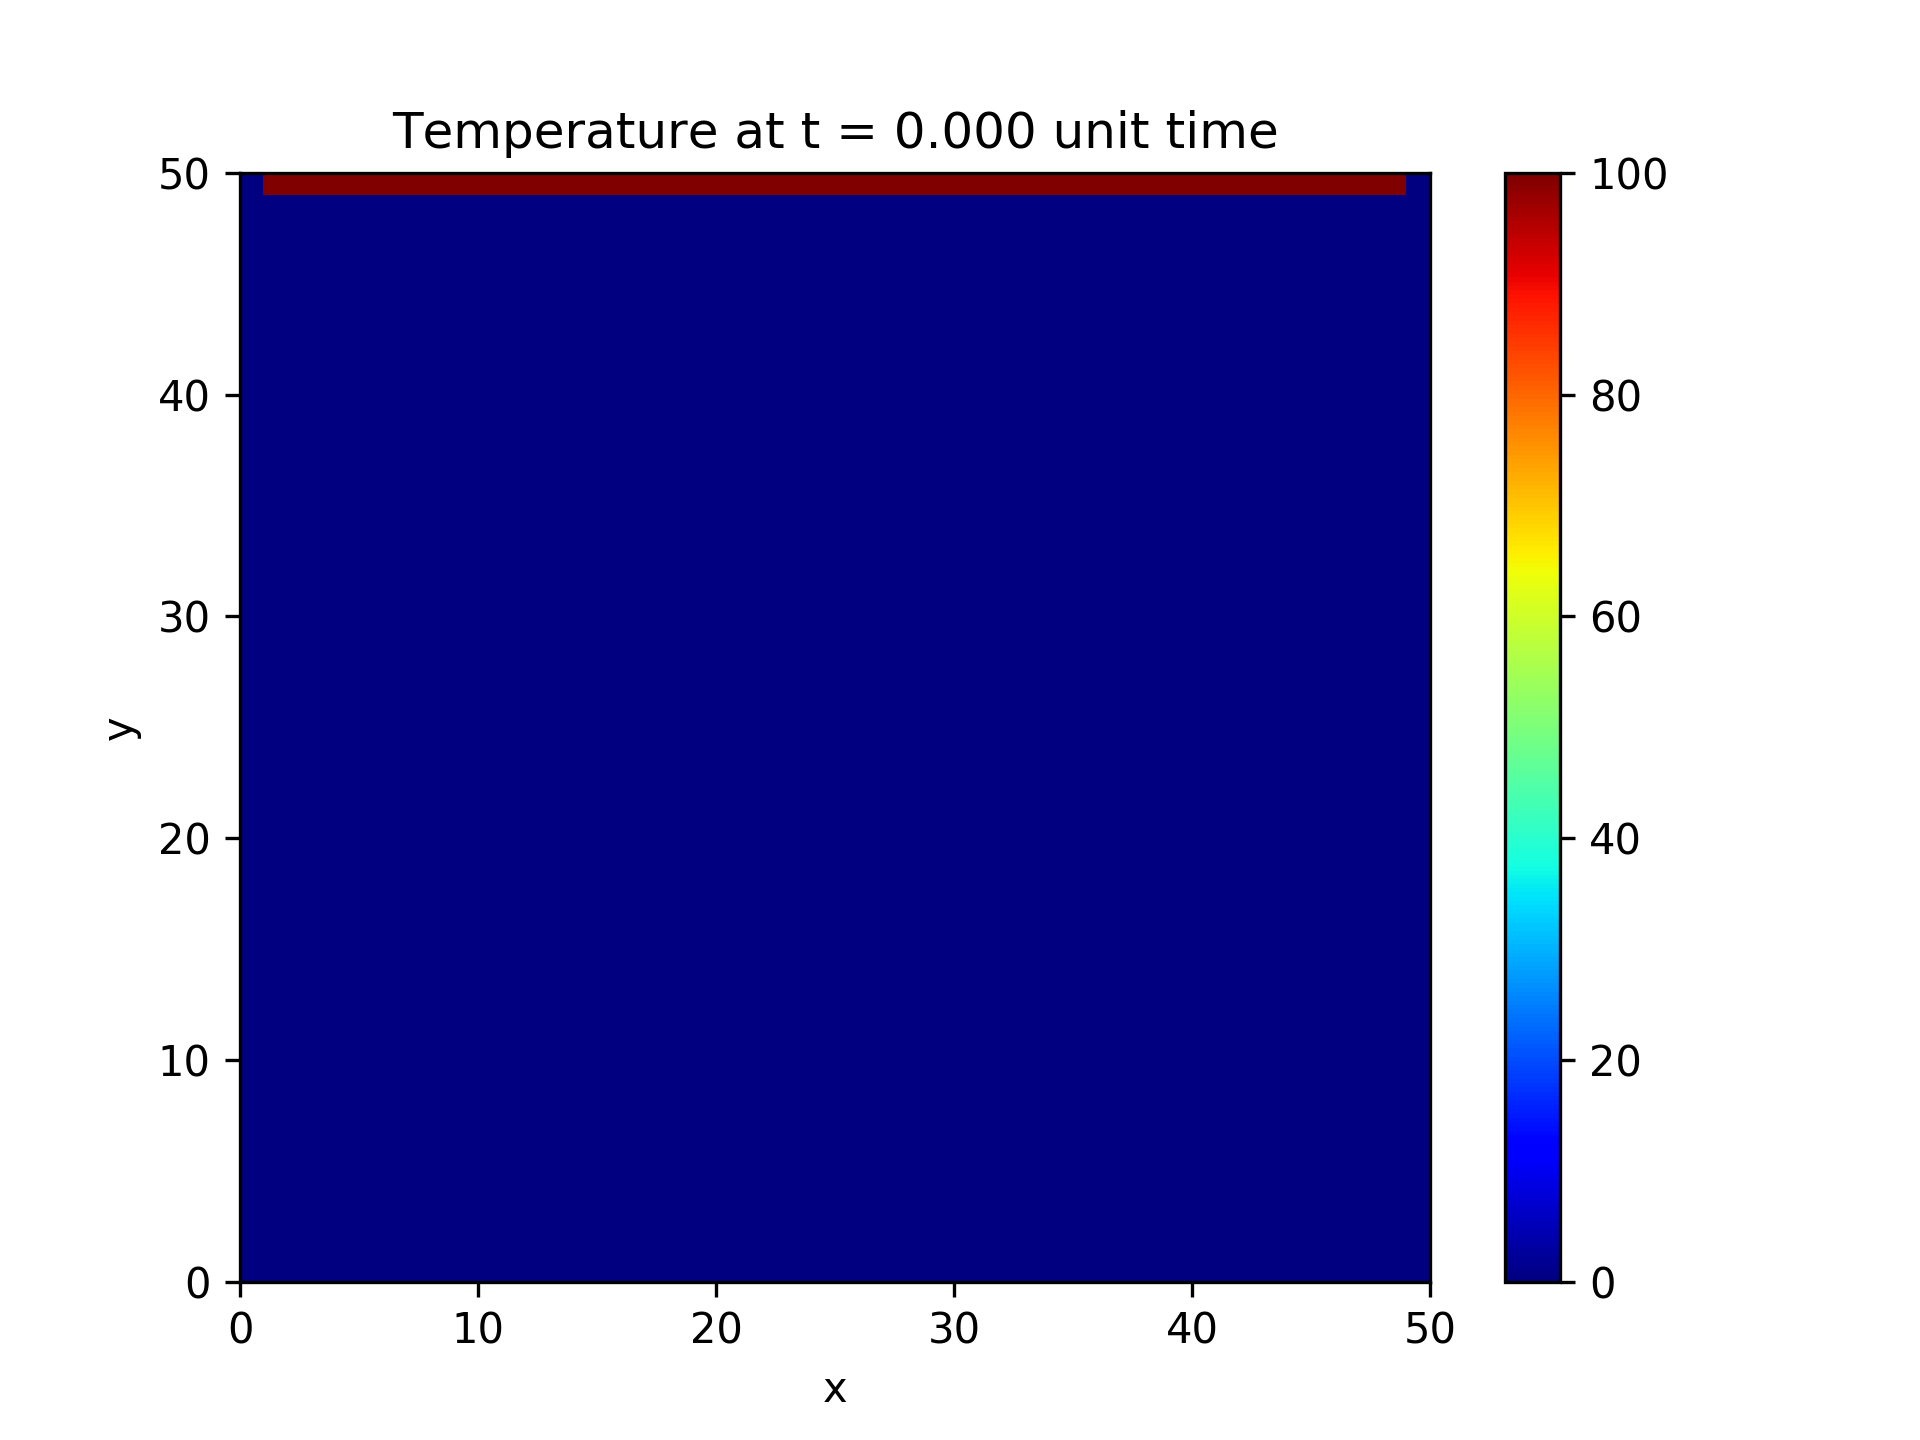
\includegraphics[width=0.7\textwidth]{figures/frame0}
	\caption{Boundary and initial conditions for our exercise.}
	\label{fig:heat_start_1}
\end{figure} 

For this example, let’s take $\Delta x = 1$ and $\alpha = 2.0$. Now we can use \texttt{python} code to solve this problem numerically to see the temperature everywhere (denoted by $i$ and $j$) and over time (denoted by $k$). 

\begin{ipython}
import numpy as np
import matplotlib.pyplot as plt

plate_length = 50
max_iter_time = 750

alpha = 2
delta_x = 1

delta_t = (delta_x ** 2)/(4 * alpha)
gamma = (alpha * delta_t) / (delta_x ** 2)

# Initialize solution: the grid of u(k, i, j)
u = np.empty((max_iter_time, plate_length, plate_length))

# Initial condition everywhere inside the grid
u_initial = 0

# Boundary conditions
u_top = 100.0
u_left = 0.0
u_bottom = 0.0
u_right = 0.0

# Set the initial condition
u.fill(u_initial)

# Set the boundary conditions
u[:, (plate_length-1):, :] = u_top
u[:, :, :1] = u_left
u[:, :1, 1:] = u_bottom
u[:, :, (plate_length-1):] = u_right

def calculate(u):
    for k in range(0, max_iter_time-1, 1):
        for i in range(1, plate_length-1, delta_x):
            for j in range(1, plate_length-1, delta_x):
                u[k + 1, i, j] = gamma * (u[k][i+1][j] + u[k][i-1][j] + 
                                          u[k][i][j+1] + u[k][i][j-1] - 
                                          4*u[k][i][j]) + u[k][i][j]

    return u

def plotheatmap(u_k, k):
    # Clear the current plot figure
    plt.clf()

    plt.title(f"Temperature at t = {k*delta_t:.3f} unit time")
    plt.xlabel("x")
    plt.ylabel("y")

    # This is to plot u_k (u at time-step k)
    plt.pcolormesh(u_k, cmap=plt.cm.jet, vmin=0, vmax=100)
    plt.colorbar()

    plt.savefig("frame"+str(k)+".png")
    return plt

# Do the calculation here
u = calculate(u)

for k in range(max_iter_time):
    plotheatmap(u[k], k)
\end{ipython}

Figure~\ref{fig:heat_end_1} shows the heat distribution after 62.5 seconds. The central part of the plate is now much warmer. 
\begin{figure}[htb]
	\centering
	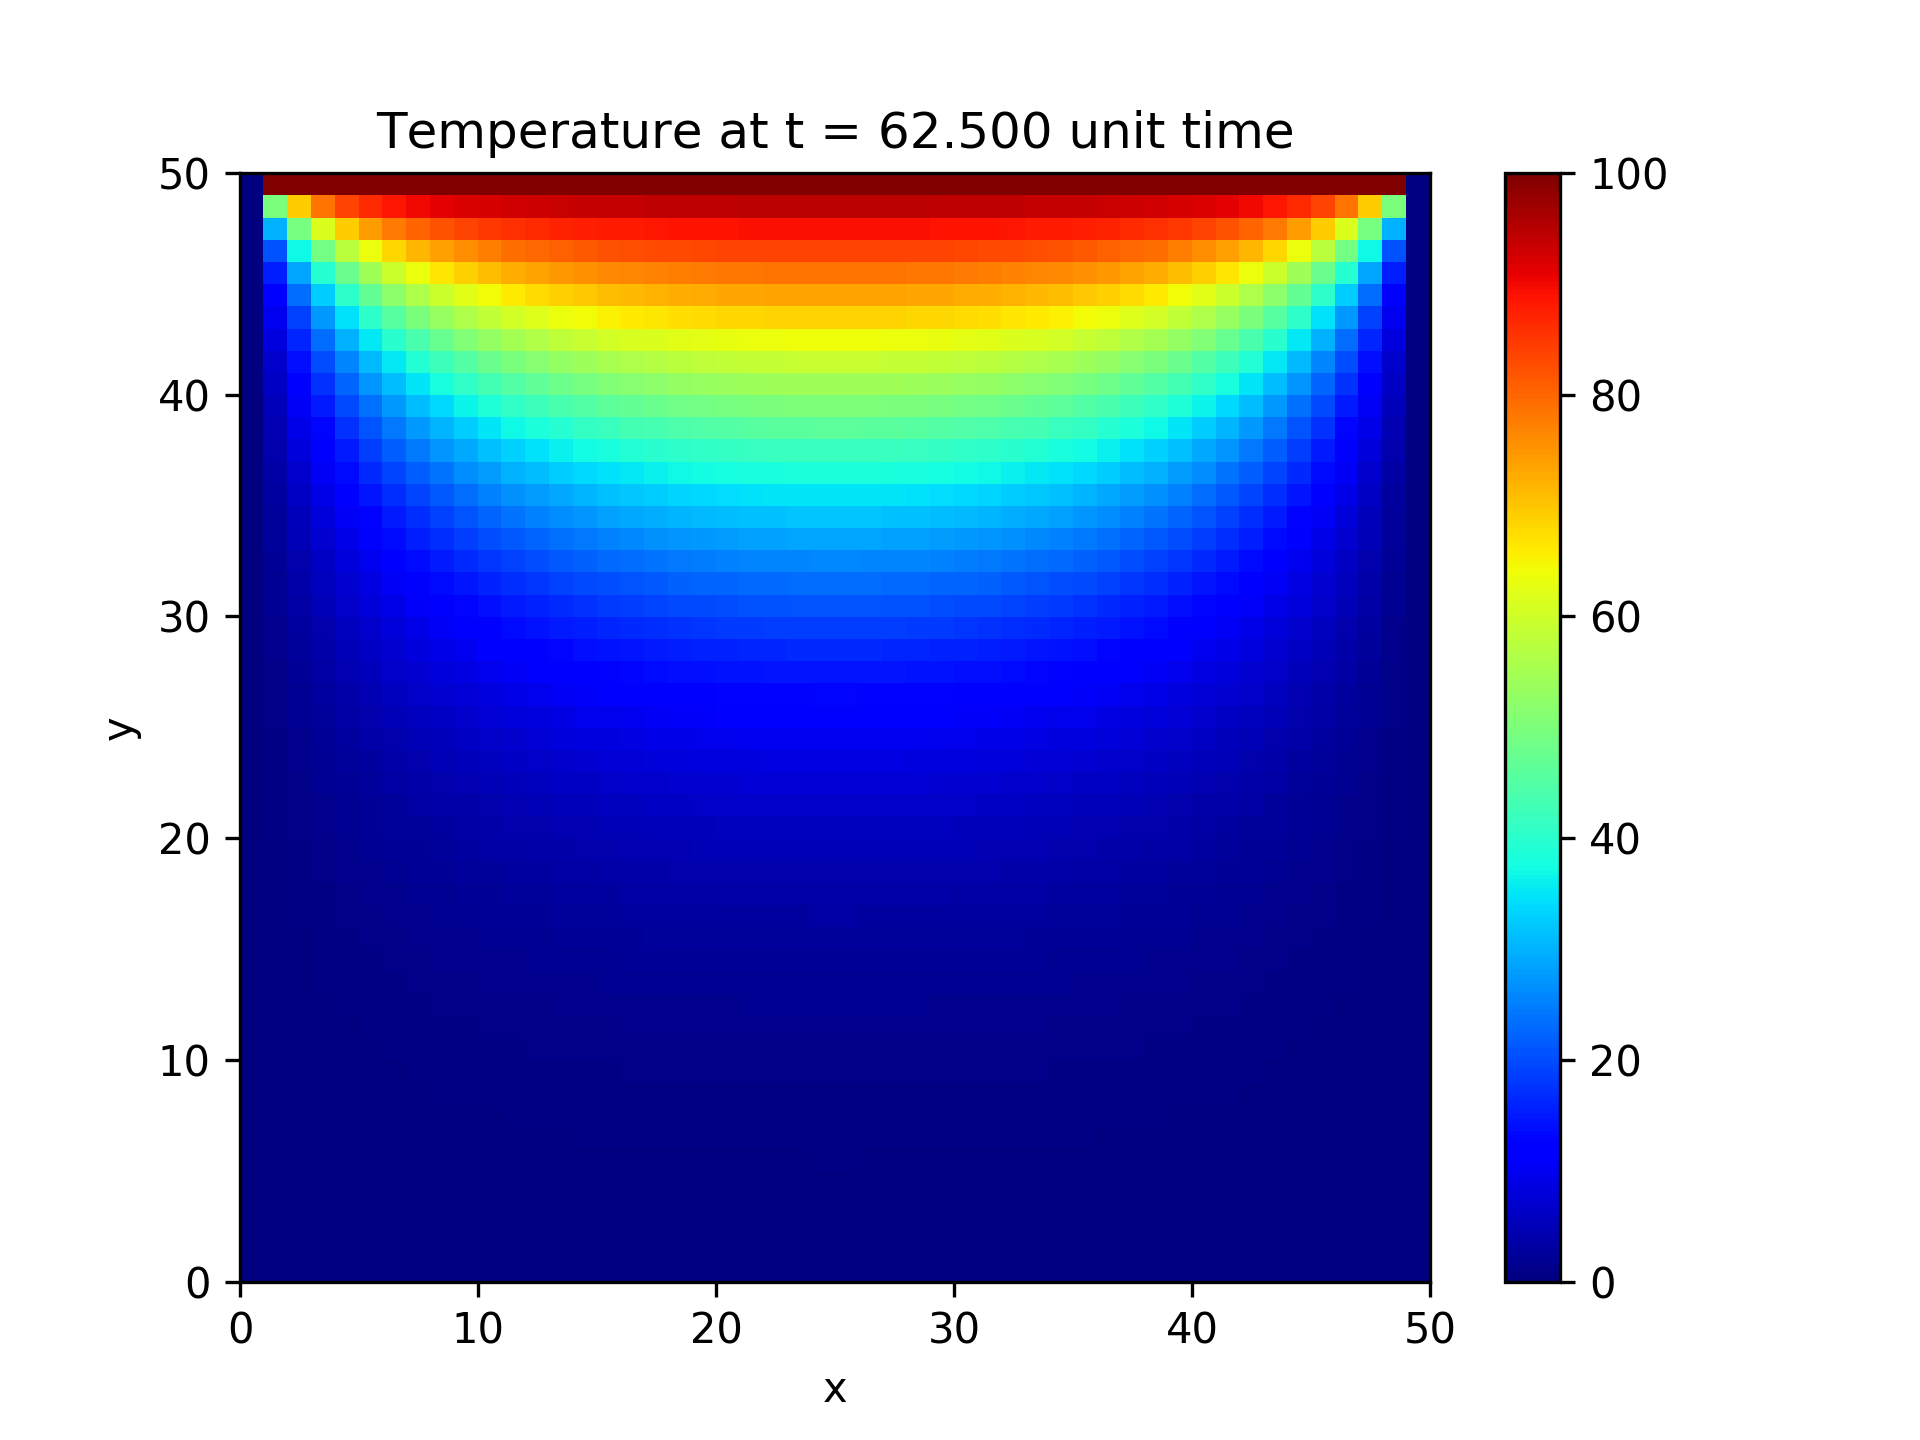
\includegraphics[width=0.7\textwidth]{figures/frame500}
	\caption{Situation after about 60 seconds.}
	\label{fig:heat_end_1}
\end{figure} 

As a second example, let’s set all of the boundary conditions to 0, and then randomize the initial condition for the interior grid (below only the new code is shown for brevity).

\begin{ipython}
...
# Initial condition everywhere inside the grid
#u_initial = 0
u_initial = np.random.uniform(low=28.5, high=55.5, size=(plate_length,plate_length))

# Change initial conditions
#u.fill(u_initial)
u[0,:,:] = u_initial

# Boundary conditions
u_top = 0.0
u_left = 0.0
u_bottom = 0.0
u_right = 0.0

# Set the initial condition
u.fill(u_initial)
...
\end{ipython}

In this second case, being the interior cools down being initially warmer than the edges of the plate. Figure~\ref{fig:heat_2} shows initial condition and the situation after 31.25 seconds.
 
\begin{figure}[htb]
	\centering
	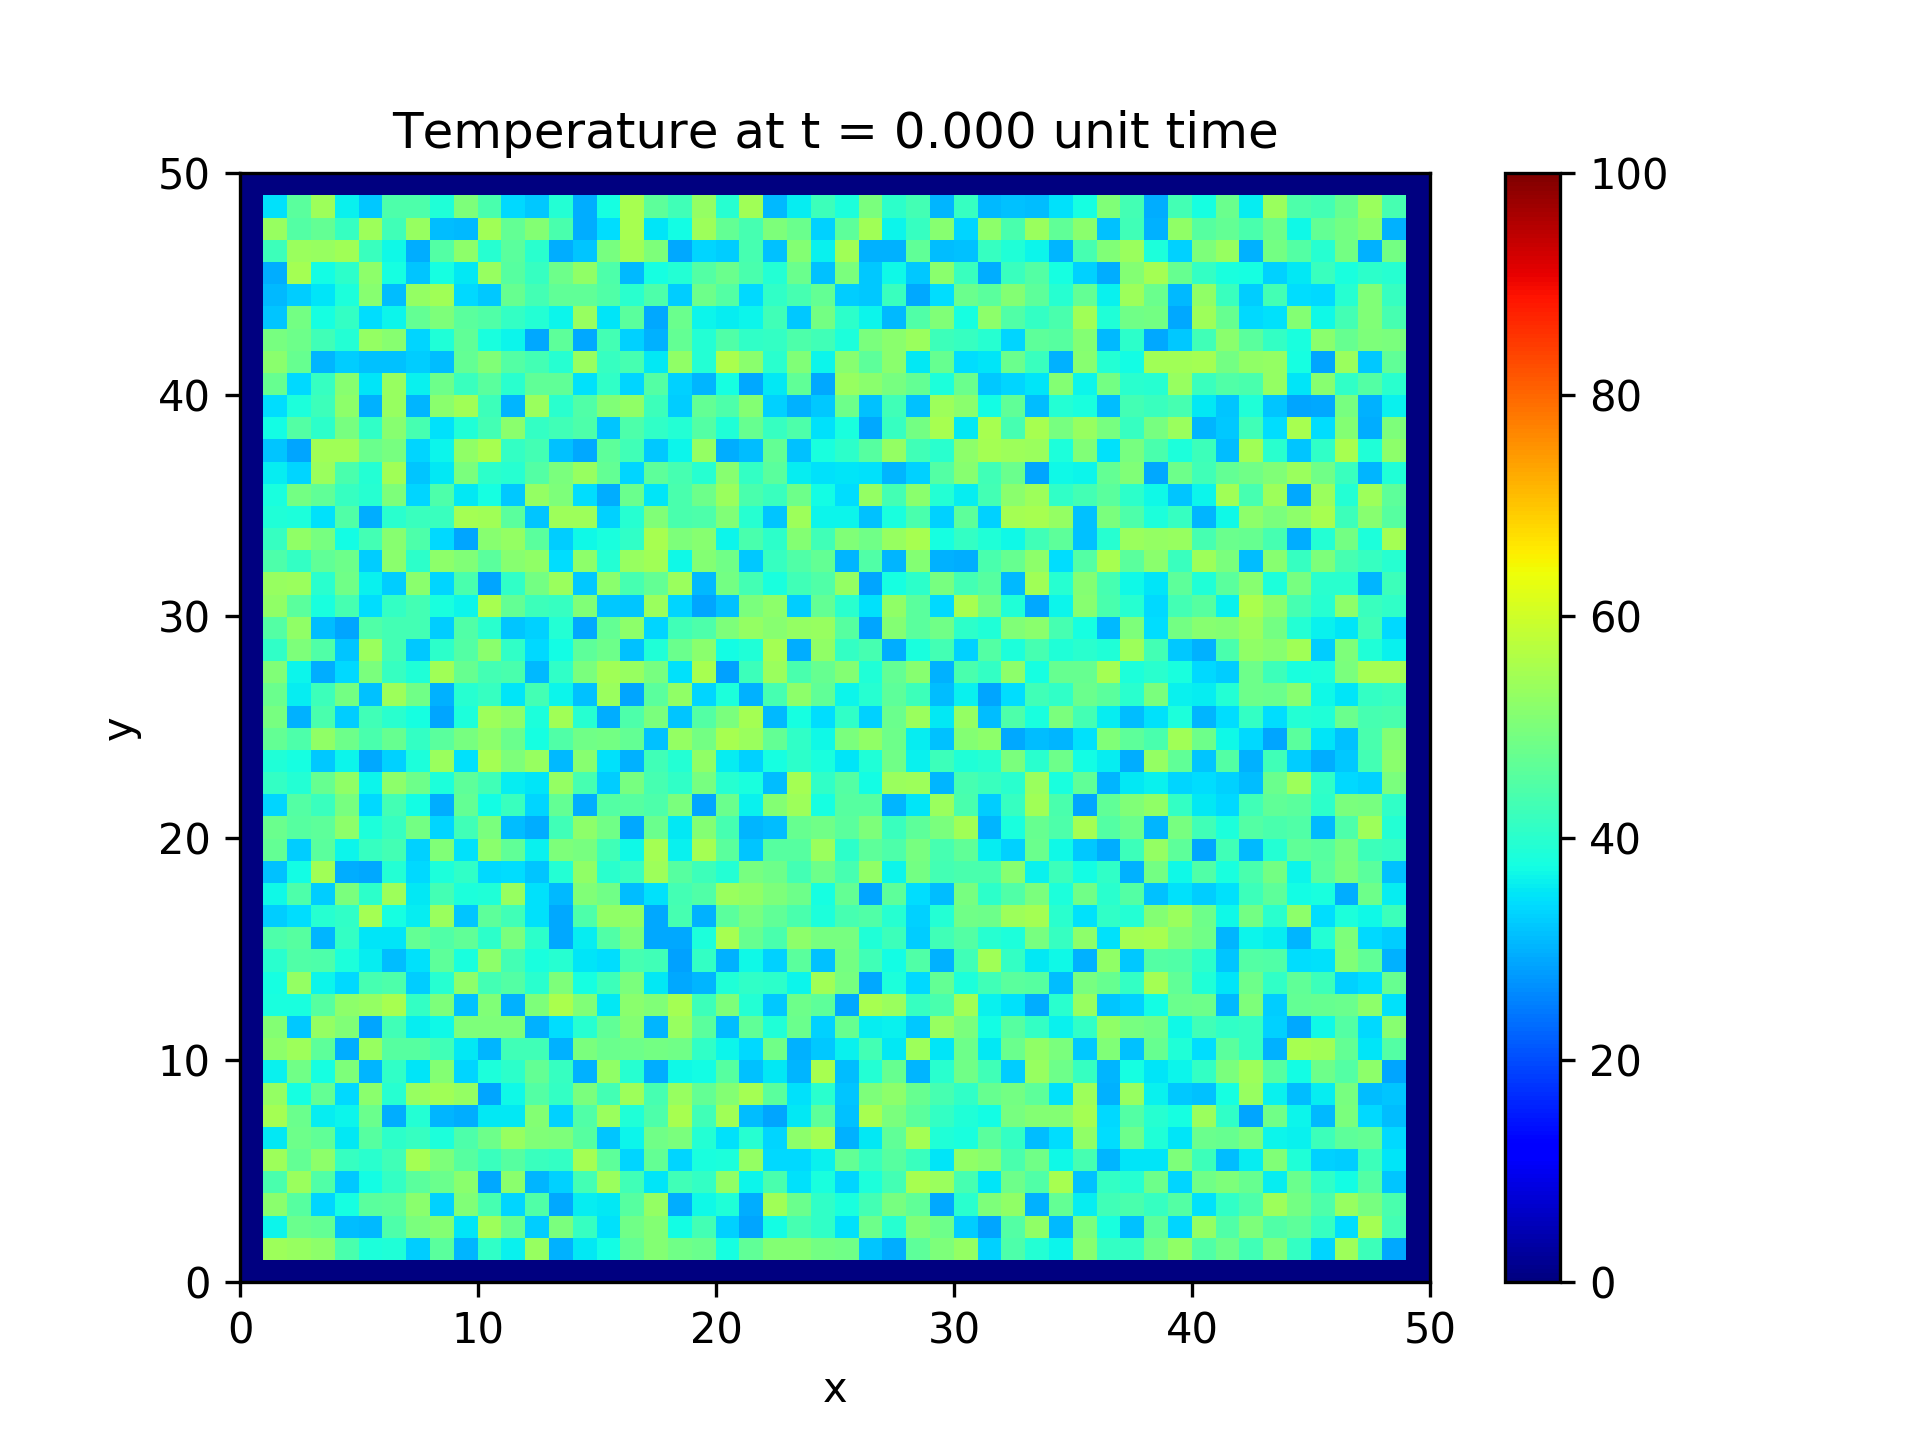
\includegraphics[width=0.45\textwidth]{figures/frame0_2}
	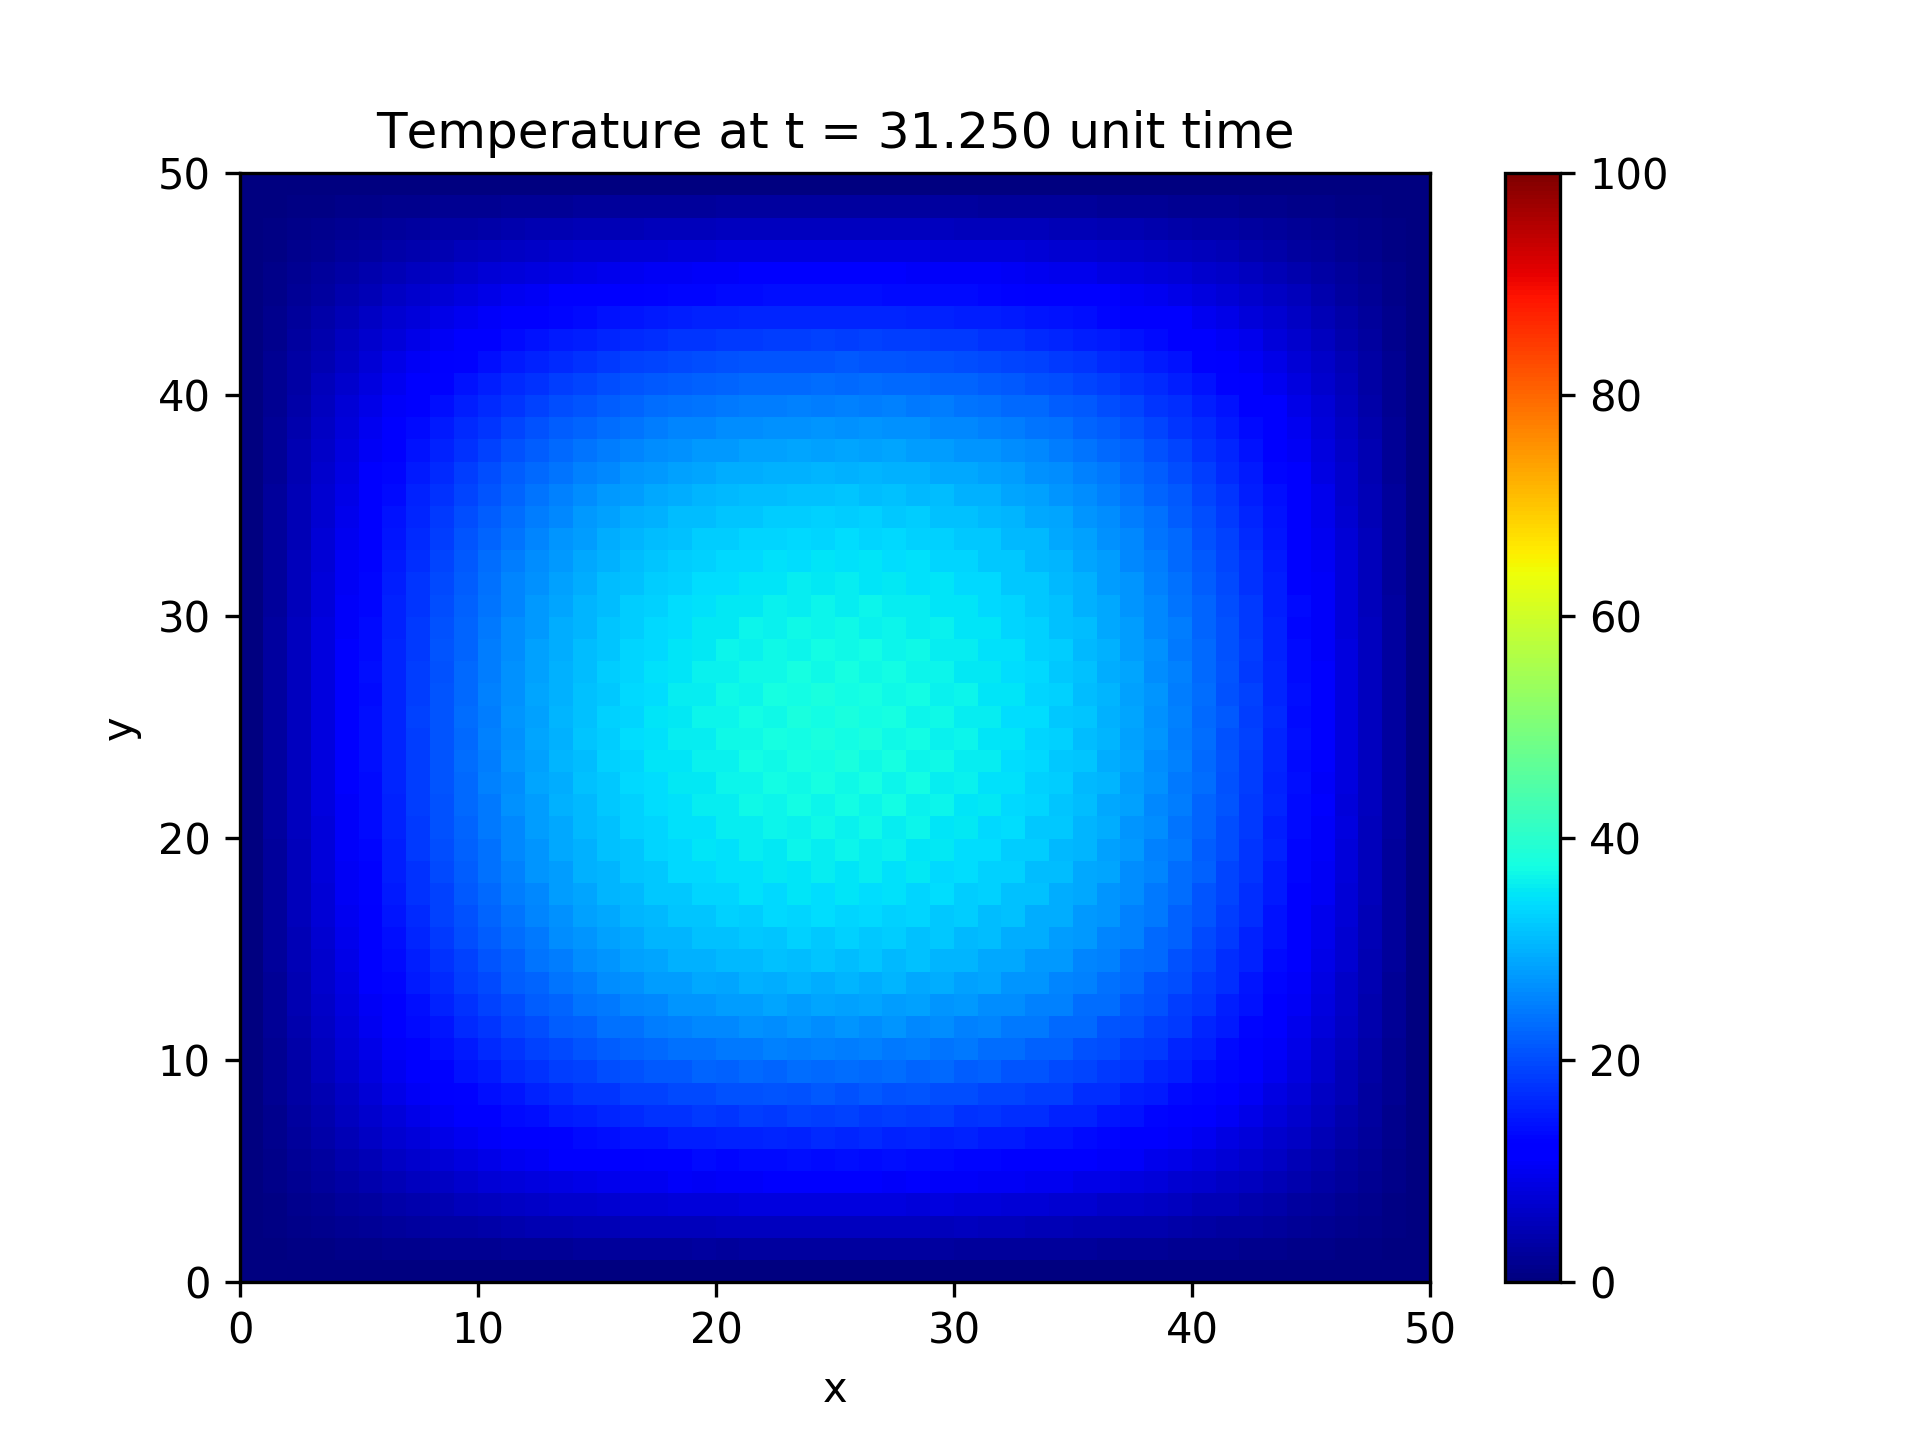
\includegraphics[width=0.45\textwidth]{figures/frame250_2}
	\caption{Initial condition of the second example of heat equation solution (left), heat distribution after  after about 30 seconds (right).}
	\label{fig:heat_2}
\end{figure} 

\section{Solving Black Scholes Equation}
Pricing an option can be done using the Black-Scholes partial differential equation (BS PDE). Here we are talking about partial differential equations since the solution will be function of more than one variables. 
The BS PDE can be derived by applying It$\hat{o}$’s Lemma to geometric Brownian motion and then setting the necessary conditions to satisfy the continuous-time delta hedging, see Chapter~\ref{ch:BS}

\begin{equation}
\cfrac{\partial V}{\partial t} + \cfrac{1}{2} \sigma^2 S^2 \cfrac{\partial^2 V}{\partial S^2}+ rS \cfrac{\partial V}{\partial S} − rV = 0
\end{equation}

We will solve this equation numerically, using \texttt{python}. The main advantage of this method is that it bypasses very complicated analytical calculations with numerical methods, which are done by our computer.

This grid will be used to simulate the PDE from point to point. The grid on the $x$-axis will represent the simulated times, which ranges from $[0,1]$ and the $y$-axis will represent the possible stock prices, ranging from $[S_{min},S_{max}]$. The result will be a 3D graph and our job is to determine the option price above each point on the grid.

To simulate on the grid we need to determine 3 boundaries (edge) conditions of the grid. In our case, we can do this for the top, the bottom, and the last boundary of the grid. The bottom is the easiest, we will set $S_{min}=0$. The top condition is a bit more tricky. It should be well above the option’s strike price $K$ to ensure the option’s value $V = \textrm{max}(S-K, 0)$ will always (with negligible probability of not happening $p < 0.0001$) payout $S-K$ . We can do this by setting $S_{max}$ 8 standard deviations away from the mean, as the stock price is log-normally distributed. So, if we take $S_{max}=8\sigma*(T-t)^{0.5}$ , we have ensured that property.
The option value $V$ at $S_{max}$ can be deducted using a replication argument. If a derivative pays $S-K$ at time $t$, we can replicate it by purchasing 1 unit of stock and putting $e^{(-r(1-t))}*K$ it into a risk-free bank account. So this makes the value of the option for large $S$: $V(t,S_{max})=S_{max} - e^{(-r(1-t))}*K$.
The final boundary condition will be the European call option’s payoff, as that will give the exact value for the option. So the three boundary conditions are

\begin{gather}
V(t, S_{min}) = 0\\
V(t,S_{max})=S_{max} - e^{(-r(1-t))}*K\\
V(1, S) = \textrm{max}(S-K, 0)
\end{gather}

In the stock price direction (vertical) we introduce $M$ points. To think about this, imagine that the possible range of $S$ is $[0,100]$ with $M=100$. This will make 100 stock points with 1 at every integer. We do the same in the time direction (horizontal) with $N$ steps. This will create a $N+1 \times  M+1$ matrix, which we can use to create derivative estimates.

\subsection{Estimating derivatives}
With the discretized space, we can use central difference estimates for the derivatives of the option value (the delta and gamma from the greeks).

\begin{gather}
\Delta = \cfrac{\partial V(t, S_i)}{\partial S} = \cfrac{V(t, S_{i+1})-V(t, S_{i-1})}{2\delta S}\\
\Gamma = \cfrac{\partial^2 V(t, S_i)}{\partial S^2} = \cfrac{V(t, S_{i+1})-2V(t, S_i) + V(t,S_{i-1})}{(\delta S)^2}
\end{gather}

Plugging these into the Black-Scholes PDE, we get
\begin{equation}
\cfrac{\partial V_i}{\partial t} + \cfrac{1}{2} \sigma^2 S_i^2 \cfrac{V(t, S_{i+1})-2V(t, S_i) + V(t,S_{i-1})}{(\delta S)^2} + rS_i \cfrac{V(t, S_{i+1})-V(t, S_{i-1})}{2\delta S} − rV_i \approx 0
\end{equation}

This can be understood easily by visualizing what the above equation does. It basically takes 3 points and calculates a weighted average of those to arrive at a point 1 step forward in time.

By iterating the above process we can simulate the above grid by going one step at a time. Note, that as we know the final boundary condition and not the first, we will be actually be going back in time.

\begin{equation}
V_{t+1} = V_t - \cfrac{1}{2} \sigma^2 S_i^2 \cfrac{V(t, S_{i+1})-2V(t, S_i) + V(t,S_{i-1})}{(\delta S)^2} - rS_i \cfrac{V(t, S_{i+1})-V(t, S_{i-1})}{2\delta S} + rV_t
\end{equation}

This is a system of ODEs, where $V$ is the column vector of option prices at each timestep. Moreover, we need to add a vector to the above equation that contains the boundary conditions at time $t$: $W_t$ , and then we can rewrite the equation in matrix notation, such that $\Lambda$ contains the multipliers. This equation now contains all the information we have and is called the explicit method. It uses the backward difference estimate for $V$ concerning $t$, which is equivalent to the forward's difference if we were simulating forward it time (we are simulating backward).

\begin{equation}
V_{t-1} \approx (1-\Lambda\delta t)V_t -\delta t W_t
\end{equation}

So, to code it up we need functions for the boundary conditions.

\section{Exercises}
\input{finite_difference_ex_text}

\begin{thebibliography}{9}
\bibitem{bib:ode}\href{https://en.wikipedia.org/wiki/Ordinary_differential_equation}{\emph{Ordinary differential equation}}, Wikipedia [Online]
\end{thebibliography}